% Algoritmy: https://docs.google.com/document/d/1cDg8dV4Rso5sAE2gYkBPsJ8a_dMLqA8MHRR1ZvceWZM/edit#heading=h.7z19cc4fgwy4
Task scheduling is one of the most important responsibilities of a task runtime, because the
quality of scheduling has an effect on the makespan of the task graph execution and also on the
achieved hardware utilization of worker nodes. It is crucial for the scheduler to be able to
distribute the tasks among all available worker nodes to achieve as much parallelization as
possible, without the induced network communication and task management overhead becoming a
bottleneck. Unfortunately, optimal task scheduling is a very difficult problem, which is NP-hard
even in the simplest cases~\cite{Ullman1975}, and there is thus no single scheduling algorithm
that could quickly provide an optimal schedule for an arbitrary task graph.

There are many factors that affect the execution properties of task graphs and that pose some form
of a challenge to task schedulers. The computational environment (e.g.\ a distributed cluster) can
have varying amounts of nodes with heterogeneous hardware resources, and complex network topologies
that can have a non-trivial effect on the latency and bandwidth of messages sent between the
workers and the scheduler, and thus in turn also on the overall performance of the task graph
execution. Task graphs can also have an arbitrarily complex structure, with large amounts of
different kinds of tasks with diverse execution characteristics and resource requirements.

Furthermore, task graph execution might not be deterministic, and the scheduler has to work with
incomplete information and react to events that dynamically occur during task execution and that
cannot be fully predicted before the task graph execution starts. The communication network can be
congested because of unrelated computations running concurrently on the cluster; tasks can also be
slowed down by congested hardware resources that can be highly non-trivial to model, such as
\gls{numa} effects, and they can also sometimes fail unpredictably and have to be
re-executed. Even the duration of each task, which is perhaps the most crucial property of a task
coveted by the scheduler, is not usually known beforehand; the most the scheduler knows about is
either an estimate from the task graph author or a running average based on historical executions
of similar tasks, both of which can be inaccurate.

In theory, all these factors should be taken into account by task scheduling algorithms. In
practice, it is infeasible to have a completely accurate model of the entire cluster, operating
system, task implementations, networking topology, etc. Therefore, task schedulers omit some of
these factors to provide a reasonable runtime performance. They rely on various heuristics with
different trade-offs that make them better suited for specific types of task graphs and
computational environments. These heuristics can suffer from non-obvious edge cases that produce
poor quality schedules or from low runtime efficiency, which can in turn erase any speedup gained
from producing a higher quality schedule.

In \gls{hpc} use-cases, the performance and quality of task scheduling is even more
important, since the scale and heterogeneity of task graphs provides an additional challenge for
the scheduler. \gls{hpc} clusters also tend to contain advanced network topologies
with low latency and high bandwidth~\cite{dragonfly,slimfly}, which offer the scheduler more leeway
to create sophisticated schedules leveraging large amounts of network communication, which would
otherwise be infeasible on clusters with slower networks.

To better understand the behavior and performance of various scheduling algorithms, and to find out
which scheduling approach is best suited for executing task graphs on distributed clusters, we have
performed an extensive analysis of several task scheduling algorithms in
\emph{Analysis of workflow schedulers in simulated distributed environments}~\cite{estee}. The two main contributions of this work are as
follows:
\begin{enumerate}
	\item We have created an extensible, open-source simulator of task graph execution, which allows users to
	      easily implement their own scheduling algorithms and compare them, while taking into account
	      various factors that affect task scheduling.
	\item We have benchmarked several task schedulers from existing literature under various conditions,
	      including factors affecting scheduling that have not been explored so far to our knowledge, like
	      the minimum delay between invoking the scheduler or the amount of knowledge about task durations
	      available to the scheduler, and evaluated the suitability of the individual algorithms for various
	      types of task graphs. All parts of the benchmark suite, including the task graphs, source codes of
	      the scheduling algorithms, the simulation environment and also benchmark scripts are provided in an
	      open and reproducible form.
\end{enumerate}

Various descriptions of schedulers, task graphs and other parts of the simulator and the benchmark
configuration used in this chapter were adapted from our publication~\cite{estee}.

\workshare{I have collaborated on this work with Ada Böhm and Vojtěch Cima, we have all contributed to it equally. Source code contribution statistics for
\estee{} can be found on GitHub\footnoteurl{https://github.com/it4innovations/estee/graphs/contributors}.}

\section{Task graph simulator}
\label{sec:estee-simulator}
To analyze scheduling algorithms, some form of an environment for executing tasks has to be used.
One possibility would be to use an actual distributed cluster, and implement multiple schedulers
into an existing task runtime. However, this approach can be expensive, both computationally
(executing a large number of task graphs with various configurations would consume a lot of cluster
computational time) and implementation-wise (adapting existing runtimes to different scheduling
algorithms is challenging). Therefore, task graph scheduling surveys tend to use some form of a
simulated environment, which simulates selected properties of a distributed cluster, and allows
comparing the performance of multiple scheduling algorithms (or other factors of a task runtime)
with a reduced accuracy, but at a fraction of the cost.

Many task scheduler surveys have been published over the years~\cite{hlfet1974, kwok1998benchmarking, hagras2003static, sinnen2005, wang2018list}, yet it is
difficult to reproduce and extend these results without having access to the exact source code used
to implement the schedulers and the simulation environment used in these surveys. As we will show
in the following chapter, the performance of scheduling algorithms can be affected by seemingly
trivial implementation details, and having access only to a high-level textual description or
pseudocode of a scheduling algorithm does not guarantee that it will be possible to reproduce it
independently with the same performance characteristics. This makes it challenging to compare
results between different simulation environments.

Apart from the environments used in existing surveys, there are also more general task simulation
environments. DAGSim~\cite{dagsim} offers a framework for comparing scheduling algorithms,
and compares the performance of a few algorithms, but does not provide its implementation, which
makes it difficult to reproduce or extend its results. SimDAG~\cite{simdag} is a task
graph simulator focused on \gls{hpc} use-cases built on top of the
SimGrid~\cite{simgrid} framework. It allows relatively simple implementation of new task
scheduling algorithms; however, it does not support any task resource requirements (e.g.\ the
number of used \gls{cpu} cores), which are crucial for simulating heterogeneous task
graphs.

In addition to simply comparing the performance of different schedulers, our goal was also to test
two factors for which we have hypothesized that they might affect scheduling; we have not seen
these explored in detail in existing works. Namely, we wanted to examine the effects of
\acrlong{msd}, the delay between two invocations of the scheduler and
\emph{information mode}, the amount of knowledge of task durations that is available to the
scheduler. These factors will be described in detail in the following section. The existing
simulation environments that we have evaluated did not have support for these factors, and it would
be non-trivial to add support for them.

To summarize, our goal was to provide a simulation environment that would be open-source,
facilitate reproducibility, support basic task resource requirements, and enable us to examine the
two mentioned factors that affect scheduling. To fulfill these goals, we have implemented a task
graph simulation framework called \estee{}. It is an \mbox{MIT-licensed}
open-source tool~\cite{estee_github} written in Python that provides an experimentation testbed
for task runtime and scheduler developers and researchers. It is flexible; it can be used to define
a cluster of workers, connect them using a configurable network model, implement a custom
scheduling algorithm and test its performance on arbitrary task graphs, with support for specifying
required \gls{cpu} core counts for individual tasks. Additionally, it comes
``battery-included''; it contains baseline implementations of several task schedulers from existing
literature and also a task graph generator that can be used to generate randomized graphs with
properties similar to real-world task graphs.

\subsection{Architecture}
\Autoref{fig:estee-architecture} shows the architecture of \estee{}. The core of the
tool is the \emph{Simulator} component, which uses discrete event
simulation~\cite{discrete_event_simulation} to simulate the execution of a task graph. It manages tasks,
queries the \emph{Scheduler} component for task-to-worker assignments (schedules) and then
assigns the tasks to their corresponding workers. The \emph{Worker} component then
simulates task execution and uses the provided network model to simulate exchanges of data (task
outputs) between individual workers of the simulated cluster.

\begin{figure}
	\centering
	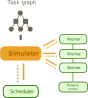
\includegraphics[scale=0.35]{estee/estee-architecture}
	\caption{\estee{} architecture}
	\label{fig:estee-architecture}
\end{figure}

\estee{} provides abstract interfaces for the task scheduler, the worker and the
network model (which simulates network communication and contention). Users can thus easily provide
their own implementations of these interfaces, and in turn override both the behavior of the
scheduler and of the cluster and its network topology.

One of our goals for \estee{} was to make it very easy to write new scheduling
algorithms and make the scheduler approachable for other researchers that might want to experiment
with task schedulers. That was also one of the motivations for deciding to create
\estee{} in Python, which facilitates experimentation. \Autoref{lst:estee-example} shows
an example of a task graph simulation that demonstrates the simplicity of defining a task graph
simulation using \estee{}. The output of the simulation is both the makespan and
also a detailed trace that can be used to visualize the individual task-to-worker assignments and
task execution time spans.

\begin{listing}
	\begin{minted}[fontsize=\normalsize]{python}
# Create task graph containing 3 tasks
# Each task runs for 1s and requires 1 CPU core
#
#     t0
#     | (50MB output)
#    / \
#  t1   t2
tg = TaskGraph()
t0 = tg.new_task(duration=1, cpus=1, output_size=50)
t1 = tg.new_task(duration=1, cpus=1)
t1.add_input(t0)
t2 = tg.new_task(duration=1, cpus=1)
t2.add_input(t0)

# Create a task scheduler
scheduler = BlevelGtScheduler()

# Define cluster with 2 workers (1 CPU core each)
workers = [Worker(cpus=1) for _ in range(2)]

# Define MaxMinFlow network model (100MB/s bandwidth)
netmodel = MaxMinFlowNetModel(bandwidth=100)

# Run simulation, return the estimated makespan in seconds
simulator = Simulator(tg, workers, scheduler, netmodel, trace=True)
makespan = simulator.run()
print(f"Task graph execution makespan = {makespan}s")
    \end{minted}
	\caption{Simple task graph simulation example using \estee{}}
	\label{lst:estee-example}
\end{listing}

\estee{} supports general task graphs represented by a \gls{dag}.
Each task has an associated duration, and can contain multiple outputs (data objects), each with an
associated size. It can also specify how many cores it requires, to model the common requirement of
executing multi-threaded functions and programs on modern \gls{hpc} machines. The
used task graph model corresponds to the task graph definition introduced
in~\Autoref{ch:taskgraphs}.

\subsection{Communication model}
Some previous scheduler surveys assume that the time to transfer a data object from one worker to
another depends merely on the size of the data object, and not on other factors, such as current
network utilization or interference~\cite{tang2010list,yao2013task,wang2018list,kwok1996dynamic}. This is an unrealistic assumption, as
the latency and bandwidth of actual computer networks is affected (among other things) by other
communication happening concurrently on the same network. Moreover, a real worker implementation
would download more than a single data object simultaneously, which further affects the transfer
durations, because the worker's bandwidth will be shared by multiple network transfers. We will use
the term \emph{communication model} and \emph{network model} interchangeably in this chapter.

We provide a more realistic network model that simulates full-duplex communication between workers,
where the total (data object) upload and download bandwidth of each worker is limited. The sharing
of bandwidth between worker connections is modeled by the
\emph{max-min fairness model}~\cite{bertsekas_1992}. Max-min fairness provides a bandwidth allocation
for each worker. If an allocation of any participant is increased, then we decrease the allocation
of some other participant with an equal or smaller allocation. When a data object transfer starts
or finishes, the data flow between workers is recomputed immediately; thus we neglect the fact that
it may take some time for the bandwidth to fully saturate.

This model is not as accurate as e.g.\ packet-level simulation implemented in some other
simulators~\cite{simgrid}, but it is a notable improvement over the naive model and it
provides reasonable runtime performance. To provide a baseline that corresponds to the naive model
described above, which has been used in several previous works, \estee{} also
implements a \emph{simple} network model. The used networking model can be configured
with an arbitrary network bandwidth amount for a given simulation.

\subsection{Scheduler parameters}
\estee{} implements support for two parameters that can affect scheduler
performance, and which we have not seen examined in detail in existing literature:
\begin{description}[wide=0pt]
	\item[\acrlong{msd}] Non-trivial schedulers create task assignments continuously during task graph execution, based on
		the current worker load and task completion times. That means that they are not invoked only once,
		but rather the task runtime invokes them repeatedly to ask them to produce assignments for tasks
		that are (or soon will be) ready to be executed at any given point in time.

		It then becomes important for a task runtime to decide when exactly it should invoke the scheduler.
		It could try to make a scheduling decision every time a task is finished; however, in practice
		there is often an upper bound on the number of scheduler invocations per second. It might be
		introduced artificially, to reduce the scheduling overhead, or it might be caused by a software or
		hardware limitation (e.g.\ messages containing task updates cannot be received more often).
		Furthermore, creating a new schedule after each task status change might not be optimal. The
		runtime can also accumulate changes for a short time period, and then provide the scheduler with a
		batch of status updates. While this increases the latency of task assignments, it can give the
		scheduler more context to work with, when it decides how it should assign tasks to workers.

		To test our hypothesis that the scheduler invocation rate can affect its performance, we introduce
		a parameter called \gls{msd}, which forces a minimal delay between two scheduler
		invocations, i.e.\ the scheduler cannot be invoked again before at least \gls{msd}
		time units have elapsed since its previous invocation.
	\item[Information mode] Many existing task scheduler descriptions assume that the duration of each task (and the size of
		each data object) is known in advance. However, this assumption is very seldom upheld when
		executing real-world task graphs. Tasks are usually specified using arbitrary function or binary
		invocations, and it is difficult to estimate their duration up front. Task runtimes thus have to
		work with completely missing information about task durations, depend on potentially imprecise user
		estimates, or calculate their own estimates based on historical task execution data. Task
		benchmarks usually use simulated task durations, which are provided to the scheduler. However, this
		might not realistically represent the scheduler's behavior for actual task graphs, for which we
		usually do not know task durations precisely before they are executed.

		We use a parameter called \emph{Information mode (imode)}, which controls the amount of knowledge the
		scheduler has of the duration of tasks. It can be set to one of the following values:
		\begin{description}
			\item[exact] The scheduler has access to the exact duration of each task and the exact size of each data object
				in the whole task graph.
			\item[user] The scheduler has access to user-defined estimations for each task in the task graph. These
				estimations are sampled from a random distribution that corresponds to a specific kind of task
				within the workflow. For example, in a task graph that performs three kinds of tasks (e.g.\
				preprocessing, computation and postprocessing), each kind of task would have its own distribution.
				We have categorized the tasks of task graphs that we have used for scheduler benchmarks described
				in~\Autoref{sec:estee-benchmarks} manually, to simulate a user that has some knowledge of the task graph
				that they are trying to compute and is able to provide some estimate of task durations and data
				object sizes.
			\item[mean] The scheduler only has access to the mean duration of all tasks and the mean size of all data
				objects in the executed task graph. This simulates a situation where a similar task graph is
				executed repeatedly, and thus there is at least some aggregated information about the task
				properties available from an earlier run.
		\end{description}
		Another possible mode to consider could be to not provide the scheduler with any task durations nor
		data object sizes in advance. This behavior would in fact correspond closely to a real-world
		execution of a task graph, where we usually do not know these task properties a priori. However, it
		is challenging to use this approach when benchmarking schedulers. Scheduler implementations are
		typically described with the assumption that task durations are known, and the scheduling
		algorithms are often fundamentally based on calculations that make use of them.

		If we took away this information, some schedulers would not be able to function, as their behavior
		is strongly influenced by an estimate of the duration of each task. Therefore, we propose using the
		\emph{mean} mode instead of not providing the scheduler with any information. We assume
		that even if the scheduler knows nothing in advance, it could always gradually record the durations
		and sizes of finished tasks, and these values would eventually converge to the global mean. In
		practice, this would take some time, while in our environment the schedulers know about the mean in
		advance. Nevertheless, as was already mentioned, we can often get a reasonable estimate of the mean
		durations based on previous executions of similar workflows.
\end{description}

%\subsection{Worker inner scheduler}
%Since each worker has to keep track of its running tasks, manage resources, and
%handle data object transfers, it becomes relatively complex. In practice, the global
%scheduler cannot micromanage each worker because this approach could not scale
%to a larger number of workers. Therefore, we model a situation where each
%worker has its own inner scheduler. We call it \emph{w-scheduler} and we
%reserve the word ``scheduler'' for the global scheduler that assigns tasks to
%workers.
%
%The w-scheduler is not a subject of study in this work, hence we are going to
%fix one particular worker scheduler and execute all experiments with it.
%The implementation is inspired by the worker implementation used in
%HyperLoom~\citep{hyperloom} and Rain. It is described in Appendix~A.

\subsection{Schedulers}
\label{subsec:estee-schedulers}
There are many task scheduling approaches, and an enormous number of various task scheduling
algorithms. We have implemented a set of task schedulers that are representatives of several common
scheduling approaches, inspired by a list of schedulers from a survey performed by Wang and
Sinnen~\cite{wang2018list}. We have included several representatives of the simplest and
perhaps most common scheduling approach, called list-scheduling, where the scheduler sorts tasks
based on some priority criteria, and then repeatedly chooses the task with the highest priority and
assigns it to a worker, which is selected by some heuristic. In addition to list-scheduling, we
have also implemented more complex approaches, such as schedulers that use work-stealing or genetic
algorithms.

Below is a list of schedulers that we have implemented and benchmarked\footnote{The labels of the individual schedulers correspond to labels used in charts that will be presented
in~\Autoref{sec:estee-benchmarks}.}:

\begin{description}[wide=0pt,itemsep=0pt,topsep=4pt]
	\item[blevel] \gls{hlfet}~\cite{hlfet1974} is a
		foundational list-based scheduling algorithm that prioritizes tasks based on their
		\emph{b-level}. B-level of a task is the length of the longest path from the task to any
		leaf task (in our case the length of the path is computed using durations of tasks, without taking
		data object sizes into account). The tasks are scheduled in a decreasing order based on their
		b-level.

	\item[tlevel]
		Smallest Co-levels First with Estimated Times~\cite{kwok1999static} is similar to
		\gls{hlfet}, with the exception that the priority value computed for each task (which is
		called \emph{t-level} here) is computed as the length of the longest path from any source
		task to the given task. This value corresponds to the earliest time that the task can start. The
		tasks are scheduled in an increasing order based on their t-level.

	\item[dls]
		Dynamic Level Scheduling~\cite{sih1993compile} calculates a dynamic level for each task-worker
		pair. It is equal to the static b-level lessened by the earliest time that the task can start on a
		given worker (considering necessary data transfers). In each scheduling step, the task-worker pair
		that maximizes this value is selected.

	\item[mcp]
		The Modified Critical Path~\cite{wu1990hypertool} scheduler calculates the ALAP
		(as-late-as-possible) time for each task. This corresponds to the latest time the task can start
		without increasing the total schedule makespan. The tasks are then ordered in ascending order based
		on this value, and scheduled to the worker that allows their earliest execution.

	\item[etf]
		The ETF (Earliest Time First) scheduler~\cite{hwang1989scheduling} selects the task-worker pair that
		can start at the earliest time at each scheduling step. Ties are broken by a higher b-level
		precomputed at the start of task graph execution.

	\item[genetic]
		This scheduler uses a genetic algorithm to schedule tasks to workers, using the mutation and
		crossover operators described in~\cite{omara2009genetic}. Only valid schedules are considered; if no
		valid schedule can be found within a reasonable number of iterations, a random schedule is
		generated instead.

	\item[ws]
		This is an implementation of a simple work-stealing algorithm. The default policy is that each task
		that is ready to be executed (all its dependencies are already computed) is always assigned to a
		worker where it can be started with a minimal transfer cost. The scheduler then continuously
		monitors the load of workers. When a worker starts to starve (and thus does not have enough tasks
		to compute), a portion of tasks assigned to other workers is rescheduled to the starving worker.
\end{description}

In addition to these schedulers, we have also implemented several naive schedulers, which serve as
a baseline for scheduler comparisons.

\begin{description}[wide=0pt]
	\item[single]
		This scheduler simply assigns all tasks to a single worker (it selects the worker with the most
		cores). The resulting schedule never induces any data transfers between workers, and does not take
		advantage of any parallelism between workers.
	\item[random]
		This scheduler simply assigns each task to a random worker using a \gls{prng} engine.
\end{description}

We have strived to implement the mentioned list-based schedulers (\emph{blevel},
\emph{tlevel}, \emph{dls}, \emph{mcp}, \emph{etf})
as closely as possible to their original description. These list-based algorithms mostly focus on
selecting the next task to schedule, but an important question (that comes up during their
implementation) is to what worker should the selected task be scheduled. The algorithm descriptions
often mention assigning the task to a worker that allows the earliest start time of the task. While
that is surely a reasonable heuristic, it is not clear how exactly such a worker should be found,
because the exact earliest start time often cannot be determined precisely in advance, since its
calculation might encompass network transfers whose duration is uncertain. This seemingly simple
implementation detail is crucial for implementing the scheduler, and it should thus be included in
the description of all scheduling algorithms that make use of such a heuristic.

\estee{} implementations of these schedulers use a simple estimation of the earliest
start time, which is based on the currently executing and already scheduled tasks of a worker and
an estimated network transfer cost based on uncontented network bandwidth (the
\emph{simple} network model is used for the scheduler's estimation of the network
transfer cost).

In order to test our hypothesis that the worker selection approach is important and affects the
scheduler's behavior, we have also created extended versions of the \emph{blevel},
\emph{tlevel} and \emph{mcp} schedulers. These modified versions use a
worker selection heuristic called ``greedy transfer``. We have not applied this heuristic to other
list-based schedulers, because it would fundamentally change their behavior.

The greedy transfer heuristic assigns the selected task to a worker that has a sufficient number of
free cores on which the task may be executed, and that requires the minimal data transfer (sum over
all sizes of data objects that have to be transferred to that worker). It also adds support for
clusters where some machines have a different number of cores than others. When a task
$t$ that needs $c$ cores cannot be scheduled because of an
insufficient number of free cores, the list-scheduling continues by taking another task in the list
instead of waiting for more free cores. This task will only consider workers that have fewer than
$c$ cores. This allows for scheduling more tasks while it does not modify the
priority of tasks because $t$ cannot be scheduled on such workers anyway. Note
that when all workers have the same number of cores, the behavior is identical to ordinary
list-scheduling.

\subsection{Task graphs}
To facilitate task scheduler experiments, \estee{} contains a task graph generator
that is able to generate parametrized instances of various categories of task graphs. Graphs from
each category can be generated using several parameters that affect their resulting size and shape.
To increase the variability of the graphs, properties like task durations or data object sizes are
sampled from a normal distribution. Below is a description of the three categories of task graphs
that can be generated:

\begin{description}[wide=0pt,itemsep=0pt,topsep=4pt]
	\item[elementary] This category contains trivial graph shapes, such as tasks with no dependencies or simple
		``fork-join'' graphs. These graphs can test the behavior of scheduler heuristics on basic task
		graph building blocks that frequently form parts of larger workflows. Examples of these graphs can
		be found in~\Autoref{app:benchmarks} (\Autoref{fig:estee-elementary-shapes}).

	\item[irw] This generator creates graphs that are inspired by real-world task graphs, such as machine-learning
		cross-validations or map-reduce workflows.

	\item[pegasus] This category is derived from graphs created by the Synthetic Workflow
		Generators~\cite{pegasusgraphs}. The generated graphs correspond to the \emph{montage},
		\emph{cybershake}, \emph{epigenomics}, \emph{ligo} and \emph{sipht}
		Pegasus workflows. The graphs have been extended with additional properties required for testing
		information modes (notably expected task durations and data object sizes for the
		\emph{user} information mode).
\end{description}

\section{Task scheduler evaluation}
\label{sec:estee-benchmarks}
We have carried out an extensive analysis of the performance of several task scheduling algorithms
on various task graphs using the \estee{} simulator. The aim of the analysis was to
explore the behavior of various schedulers in a complex simulation environment. In addition to
comparing the schedulers among each other, we also wanted to test how their performance differs
between various communication models and scheduler parameters.

Note that since the used simulation environment is focused on simulating different task graph
schedules and network transfers, and it does not model the actual execution of the scheduler nor
the task runtime in a cycle-accurate way, the term \emph{scheduler performance} refers to the simulated
makespan of task graphs executed using schedules provided by the given scheduler. In other words,
our experiments estimate how quickly a given task graph would be fully computed on a cluster, using
a given network model, while being scheduled by a specific scheduling algorithm.

\subsection{Benchmark configuration}
Below, you can find descriptions of the cluster, scheduler and task graph configurations that we
have used for our benchmarks.

\begin{description}[wide=0pt,itemsep=0pt,topsep=4pt]
	\item[Task graphs] The \estee{} graph generators were used to generate a collection of task graphs that
		were used in the benchmarks. The properties of all used graphs are summarized
		in~\Autoref{app:benchmarks} (\Autoref{tab:estee-graph-properties}). The generated task graph dataset is available as a reproducible
		artifact~\cite{estee_graphs}.
	\item[Schedulers] We have benchmarked all schedulers described in~\Autoref{subsec:estee-schedulers}. Schedulers that use the
		greedy transfer heuristic are labeled in the benchmark results with a \emph{-gt}
		suffix.
	\item[Scheduler parameters] To evaluate the effect of minimal scheduling delay, we have used a baseline value of zero, where
		the scheduler is invoked immediately after any task status update, and then a delay of
		$0.1$, $0.4$, $1.6$ and $6.4$
		seconds. In the cases where \gls{msd} is non-zero, we have also added a
		$50$ milliseconds delay before sending the scheduler decision to workers, to
		simulate the time taken by the scheduler to produce the schedule. For experiments that do not focus
		on \gls{msd}, we always use an \gls{msd} of $0.1$ seconds
		and the $50$ milliseconds computation delay. To evaluate information modes, we
		have used the \emph{exact}, \emph{user} and \emph{mean} imodes. For
		experiments that do not focus on imodes, we always use the \emph{exact} mode.
	\item[Network models] The simple (labeled \emph{simple}) and max-min (labeled \emph{max-min}) network
		models were used, with bandwidth speeds ranging from \SI{32}{\mebi\byte}/s to
		\SI{8}{\gibi\byte}/s. For experiments that do not focus on the network model (e.g.\ when imodes
		are being compared), we always use the \emph{max-min} network model.
	\item[Clusters] We have used the following five cluster (worker) configurations (where $w \times c$ means
		that the cluster has $w$ workers and each worker has $c$
		cores):  8$\times$4, 16$\times$4, 32$\times$4,
		16$\times$8, 32$\times$16.
\end{description}

\subsection{Evaluation}
This section discusses selected results of the described benchmarks. Complete benchmark results and
overview charts can be found in~\cite{estee}. The benchmarking environment, input task
graph datasets, all benchmark configurations, results and charts are also freely available as
reproducible artifacts~\cite{estee_results} for further examination.

The benchmarks were executed on the clusters of the IT4Innovations supercomputing
center~\cite{it4i}. The actual characteristics of the cluster hardware is not
important, because all benchmarks were executed using the \estee{} simulator, so the
benchmark results do not depend on the used hardware. Each benchmark that was non-deterministic in
any way (e.g.\ because it used a pseudo-random number generator) was executed twenty times. Unless
otherwise specified, the individual experiments were performed with the default benchmark
configuration that uses the \emph{max-min} network model, the \emph{exact}
information mode and a \acrlong{msd} of \SI{0.1}{\second}.

Note that the vertical axis of some charts presented in this section does not start at zero, as the
goal was to focus on the relative difference between different scheduling algorithms rather than on
the absolute makespan durations.

\subsubsection*{Random scheduler}

\begin{figure}
	\centering
	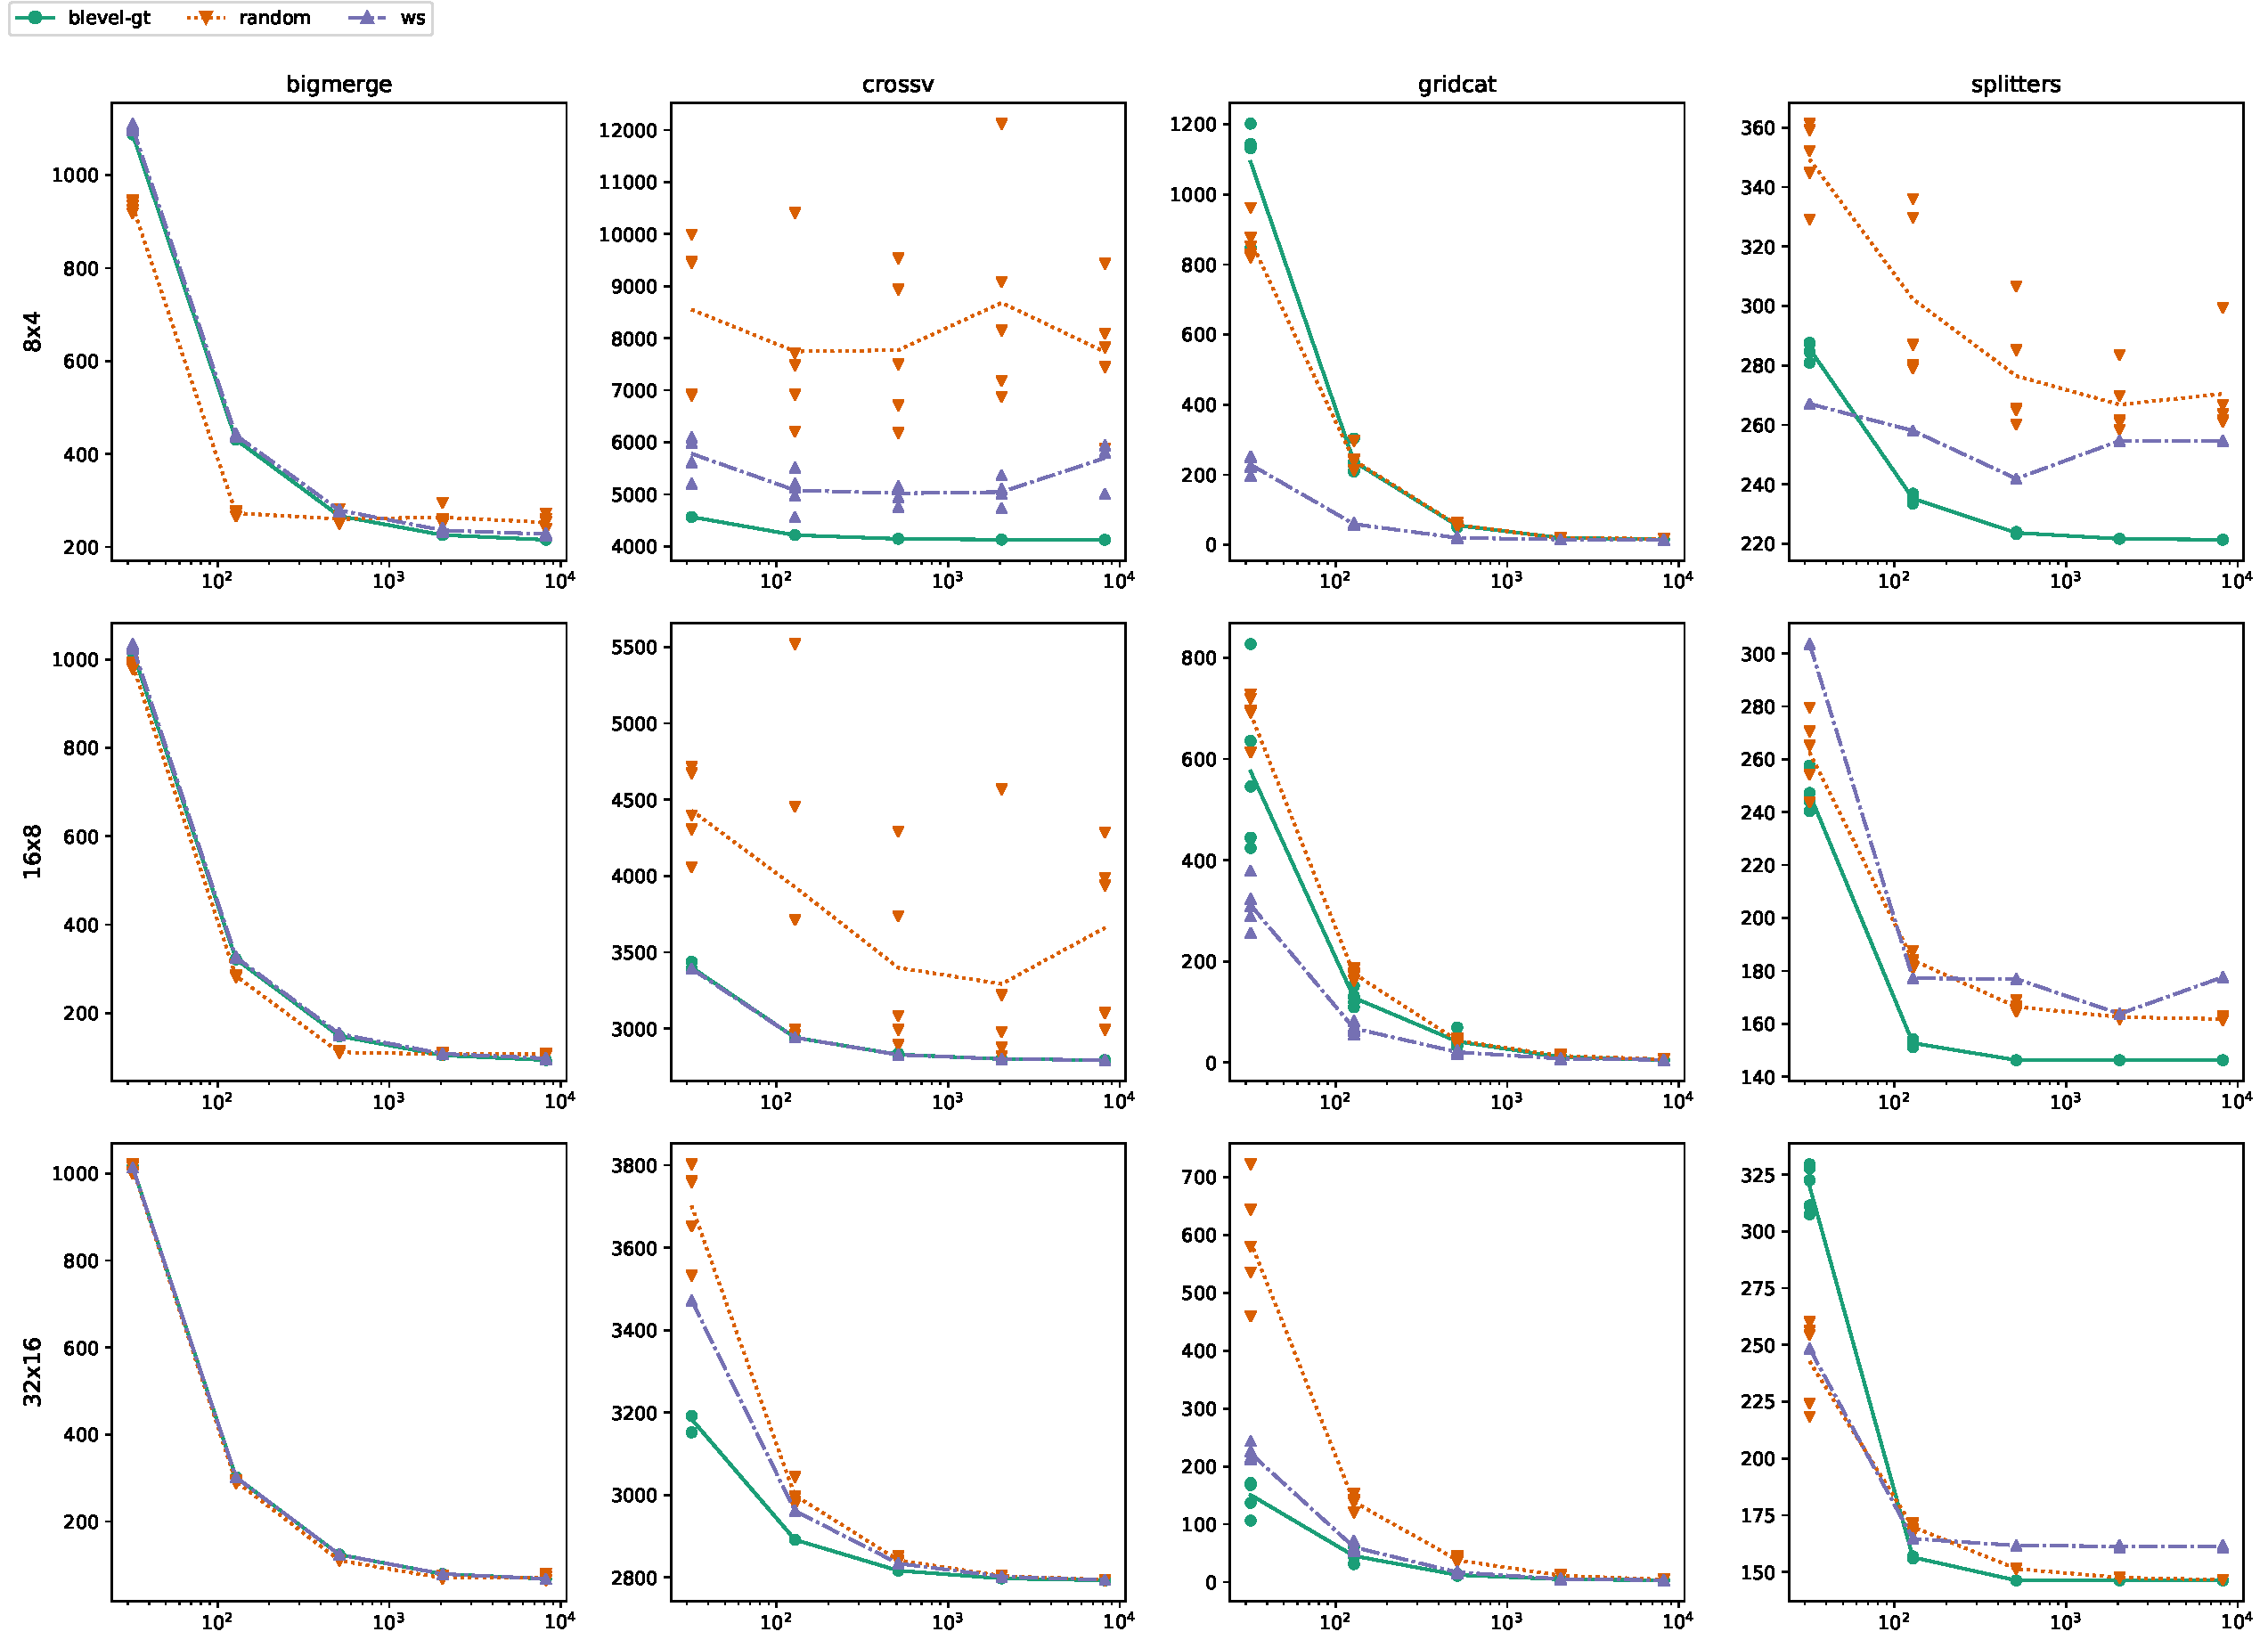
\includegraphics[width=\textwidth]{imgs/estee/charts/random-scheduler}\\
	{\small horizontal axis: bandwidth [MiB/s]; vertical axis: makespan [s]; row: cluster}
	\caption{Performance of the \emph{random} scheduler}
	\label{fig:estee-chart-random-scheduler}
\end{figure}

Given the fact that task scheduling is an NP-hard problem, it would seem that a random scheduling
approach should produce unsatisfying results. Therefore, we wanted to examine how a completely random
scheduler holds up against more sophisticated approaches. \Autoref{fig:estee-chart-random-scheduler} compares the
simulated makespan durations of the \emph{random} scheduler vs. two other competitive
schedulers (\emph{blevel-gt} and the work-stealing \emph{ws} scheduler) on
several task graphs.

While there are indeed cases where random scheduling falls short (for example on the
cross-validation \emph{crossv} task graph, or in situations with many workers and a slow
network), in most cases its performance is similar to other schedulers, and in a few situations it
even surpasses them. Its performance improves with increasing worker count and network speed. This
makes intuitive sense, because if there are enough workers and the network is fast enough to
overcome the cost of exchanging many data objects between them, the specific assignment of tasks
between workers becomes less important. As long as the scheduler is able to keep the workers busy
(which can be ensured even by a random schedule for some task graphs), then the resulting
performance might be reasonable.

We have been able to validate these results in~\cite{rsds}, where we have shown that as
the worker count becomes larger, scheduling decisions can in some cases become less important, and
other factors (like the overhead of the task runtime) might start to dominate the overall task
graph execution cost. This will be described in more detail in~\Autoref{ch:rsds}.

\subsubsection*{Worker selection strategy}

\begin{figure}
	\centering
	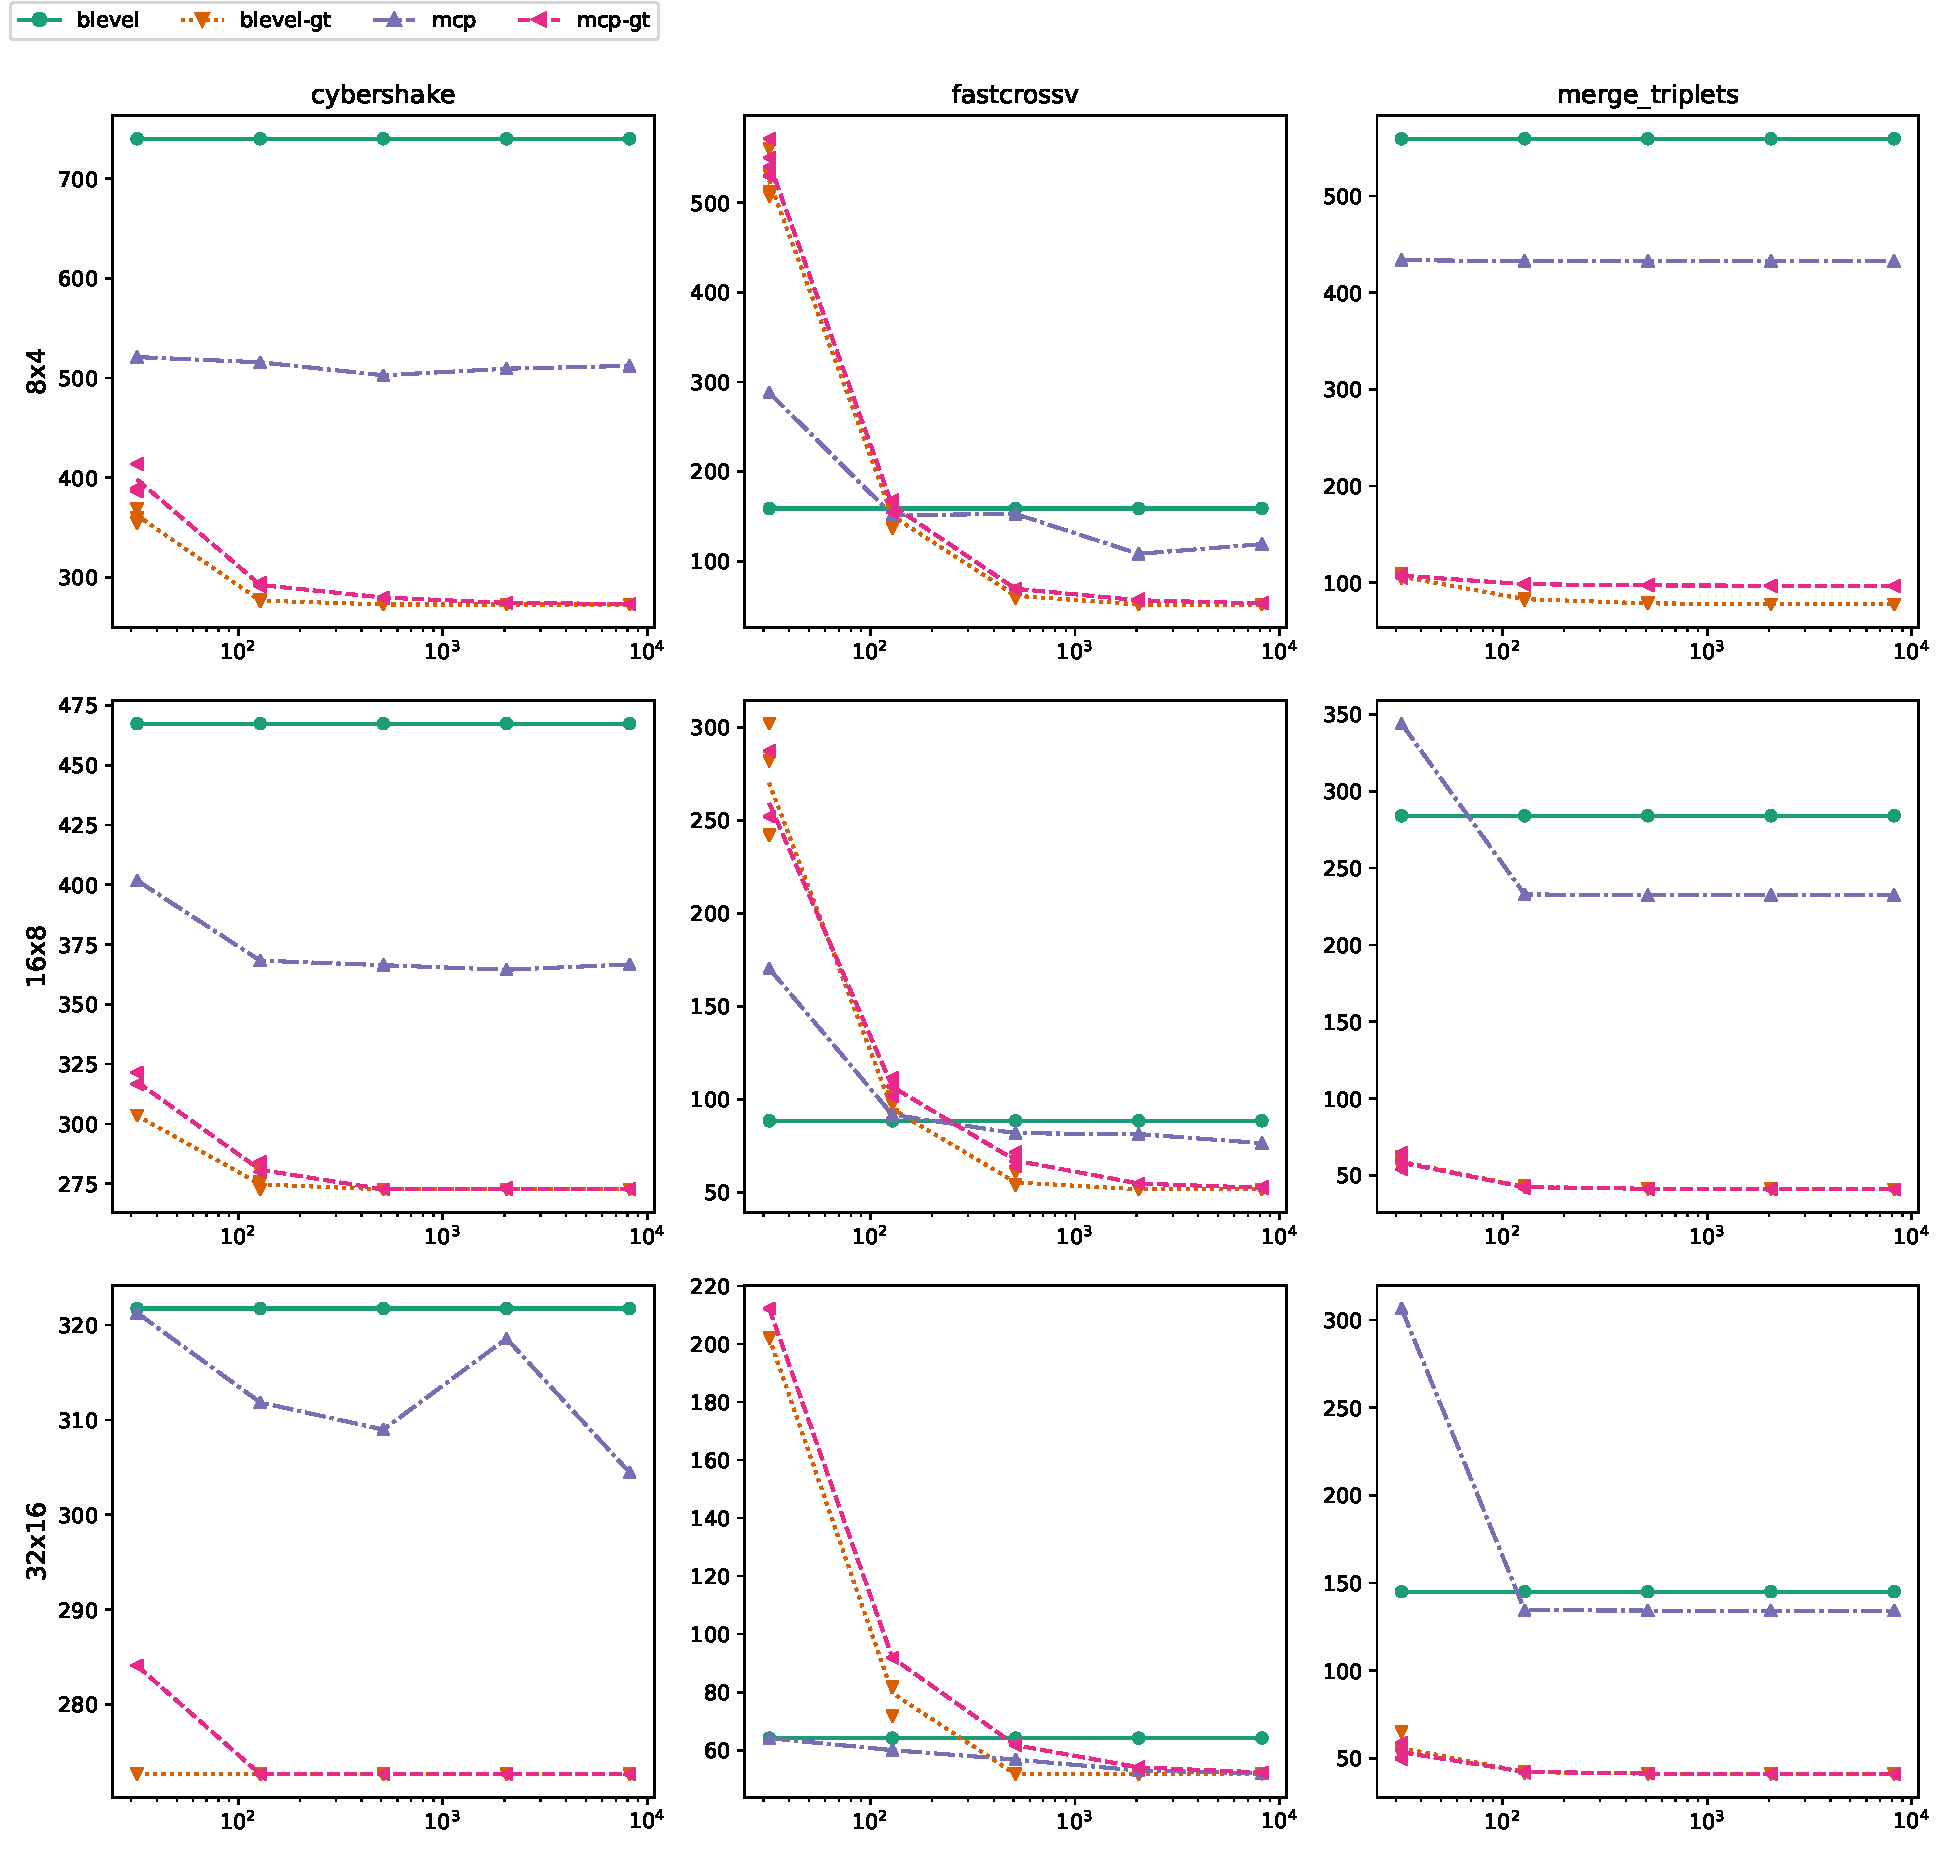
\includegraphics[width=0.8\textwidth]{imgs/estee/charts/gt-scheduler}\\
	{\small horizontal axis: bandwidth [MiB/s]; vertical axis: makespan [s]; row: cluster}
	\caption{Comparison of worker selection strategy}
	\label{fig:estee-chart-gt-scheduler}
\end{figure}

As was explained in~\Autoref{subsec:estee-schedulers}, the descriptions of several schedulers that we have
implemented in~\estee{} do not specify the concrete strategy for selecting a worker
that can start executing a given task as soon as possible. Yet, as we can see
in~\Autoref{fig:estee-chart-gt-scheduler}, this implementation detail is crucial. This chart shows the performance
of two scheduling algorithms (\emph{blevel} and \emph{mcp}), each in two
variants, with the simple selection strategy and with the greedy transfer strategy (the used worker
selection strategy was the only difference between the simple and the \emph{-gt}
suffixed variants).

It can be seen that there is a large difference between these two strategies. In fact, the results
suggest that in these specific scenarios, the worker selection strategy had a larger effect on the
overall performance than the used scheduling (task selection) algorithm, as the variants using
greedy transfer were highly correlated. This suggests that the used worker selection strategy is an
important detail of list-scheduling algorithms that should not be omitted from their descriptions.

\subsubsection*{Network models}

\begin{figure}
	\centering
	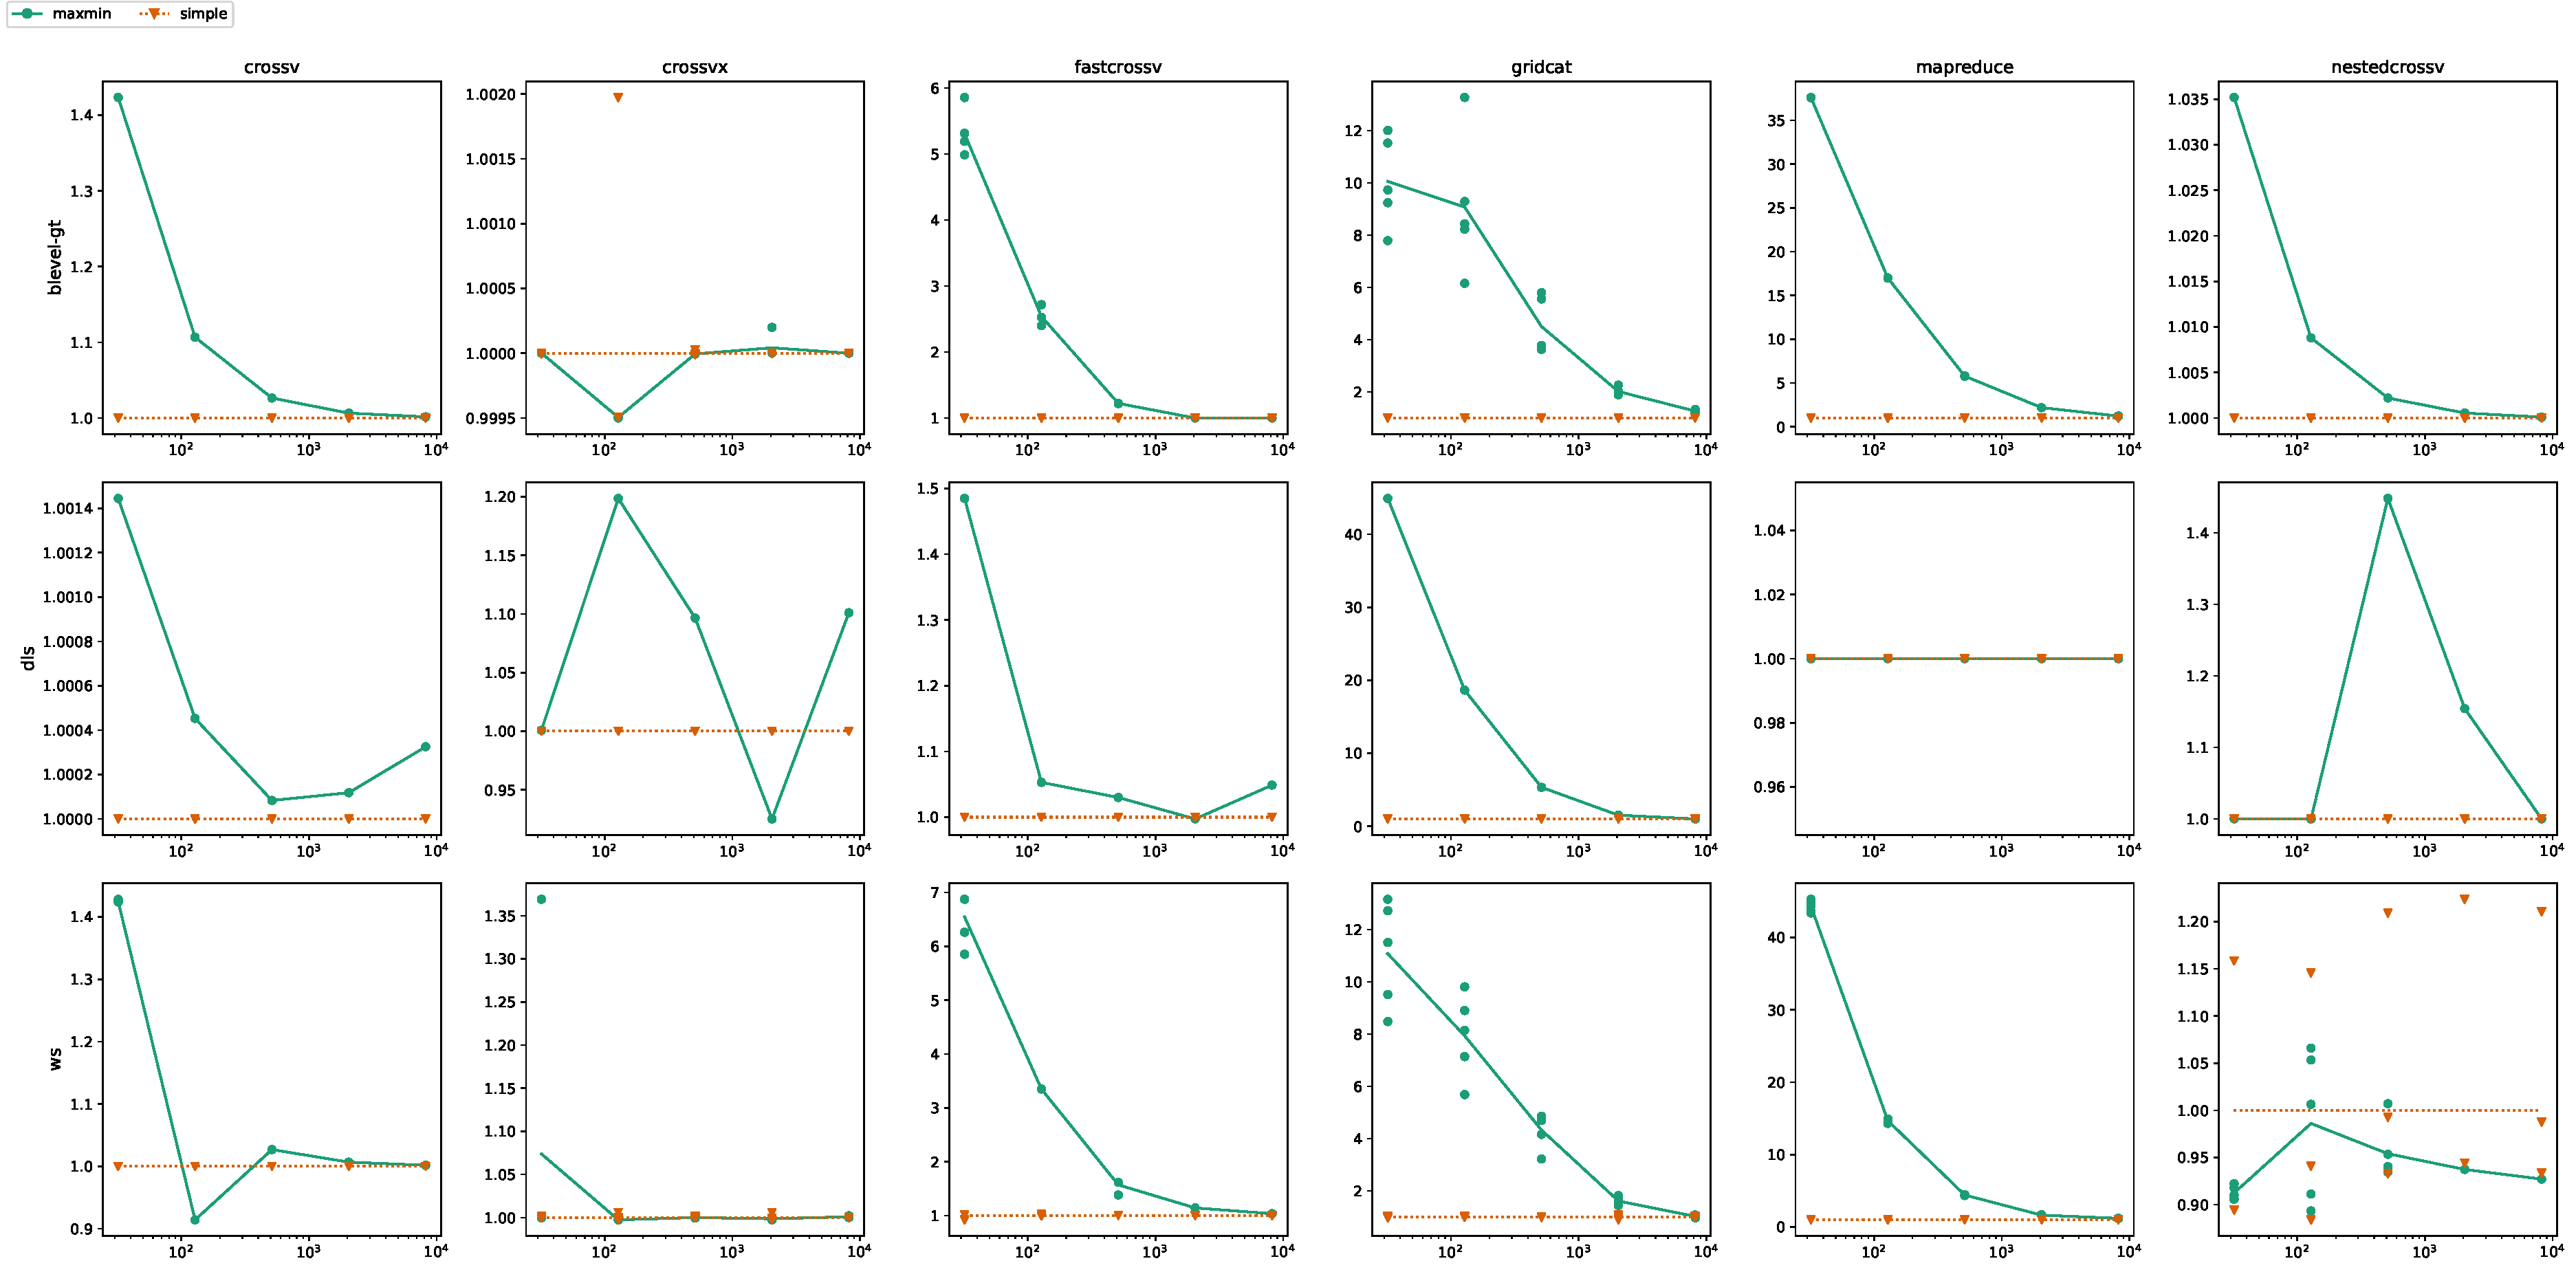
\includegraphics[width=\textwidth]{imgs/estee/charts/irw-32x4-netmodel-score}\\
	{\small horizontal axis: bandwidth [MiB/s]; vertical axis: makespan normalized to average
	of the \emph{simple} model; row: scheduler; cluster $32x4$}
	\caption{Comparison of \emph{max-min} and \emph{simple} network models
	(\emph{irw} dataset)} \label{fig:estee-chart-irw-netmodel}
\end{figure}

%\begin{figure}
%	\centering
%	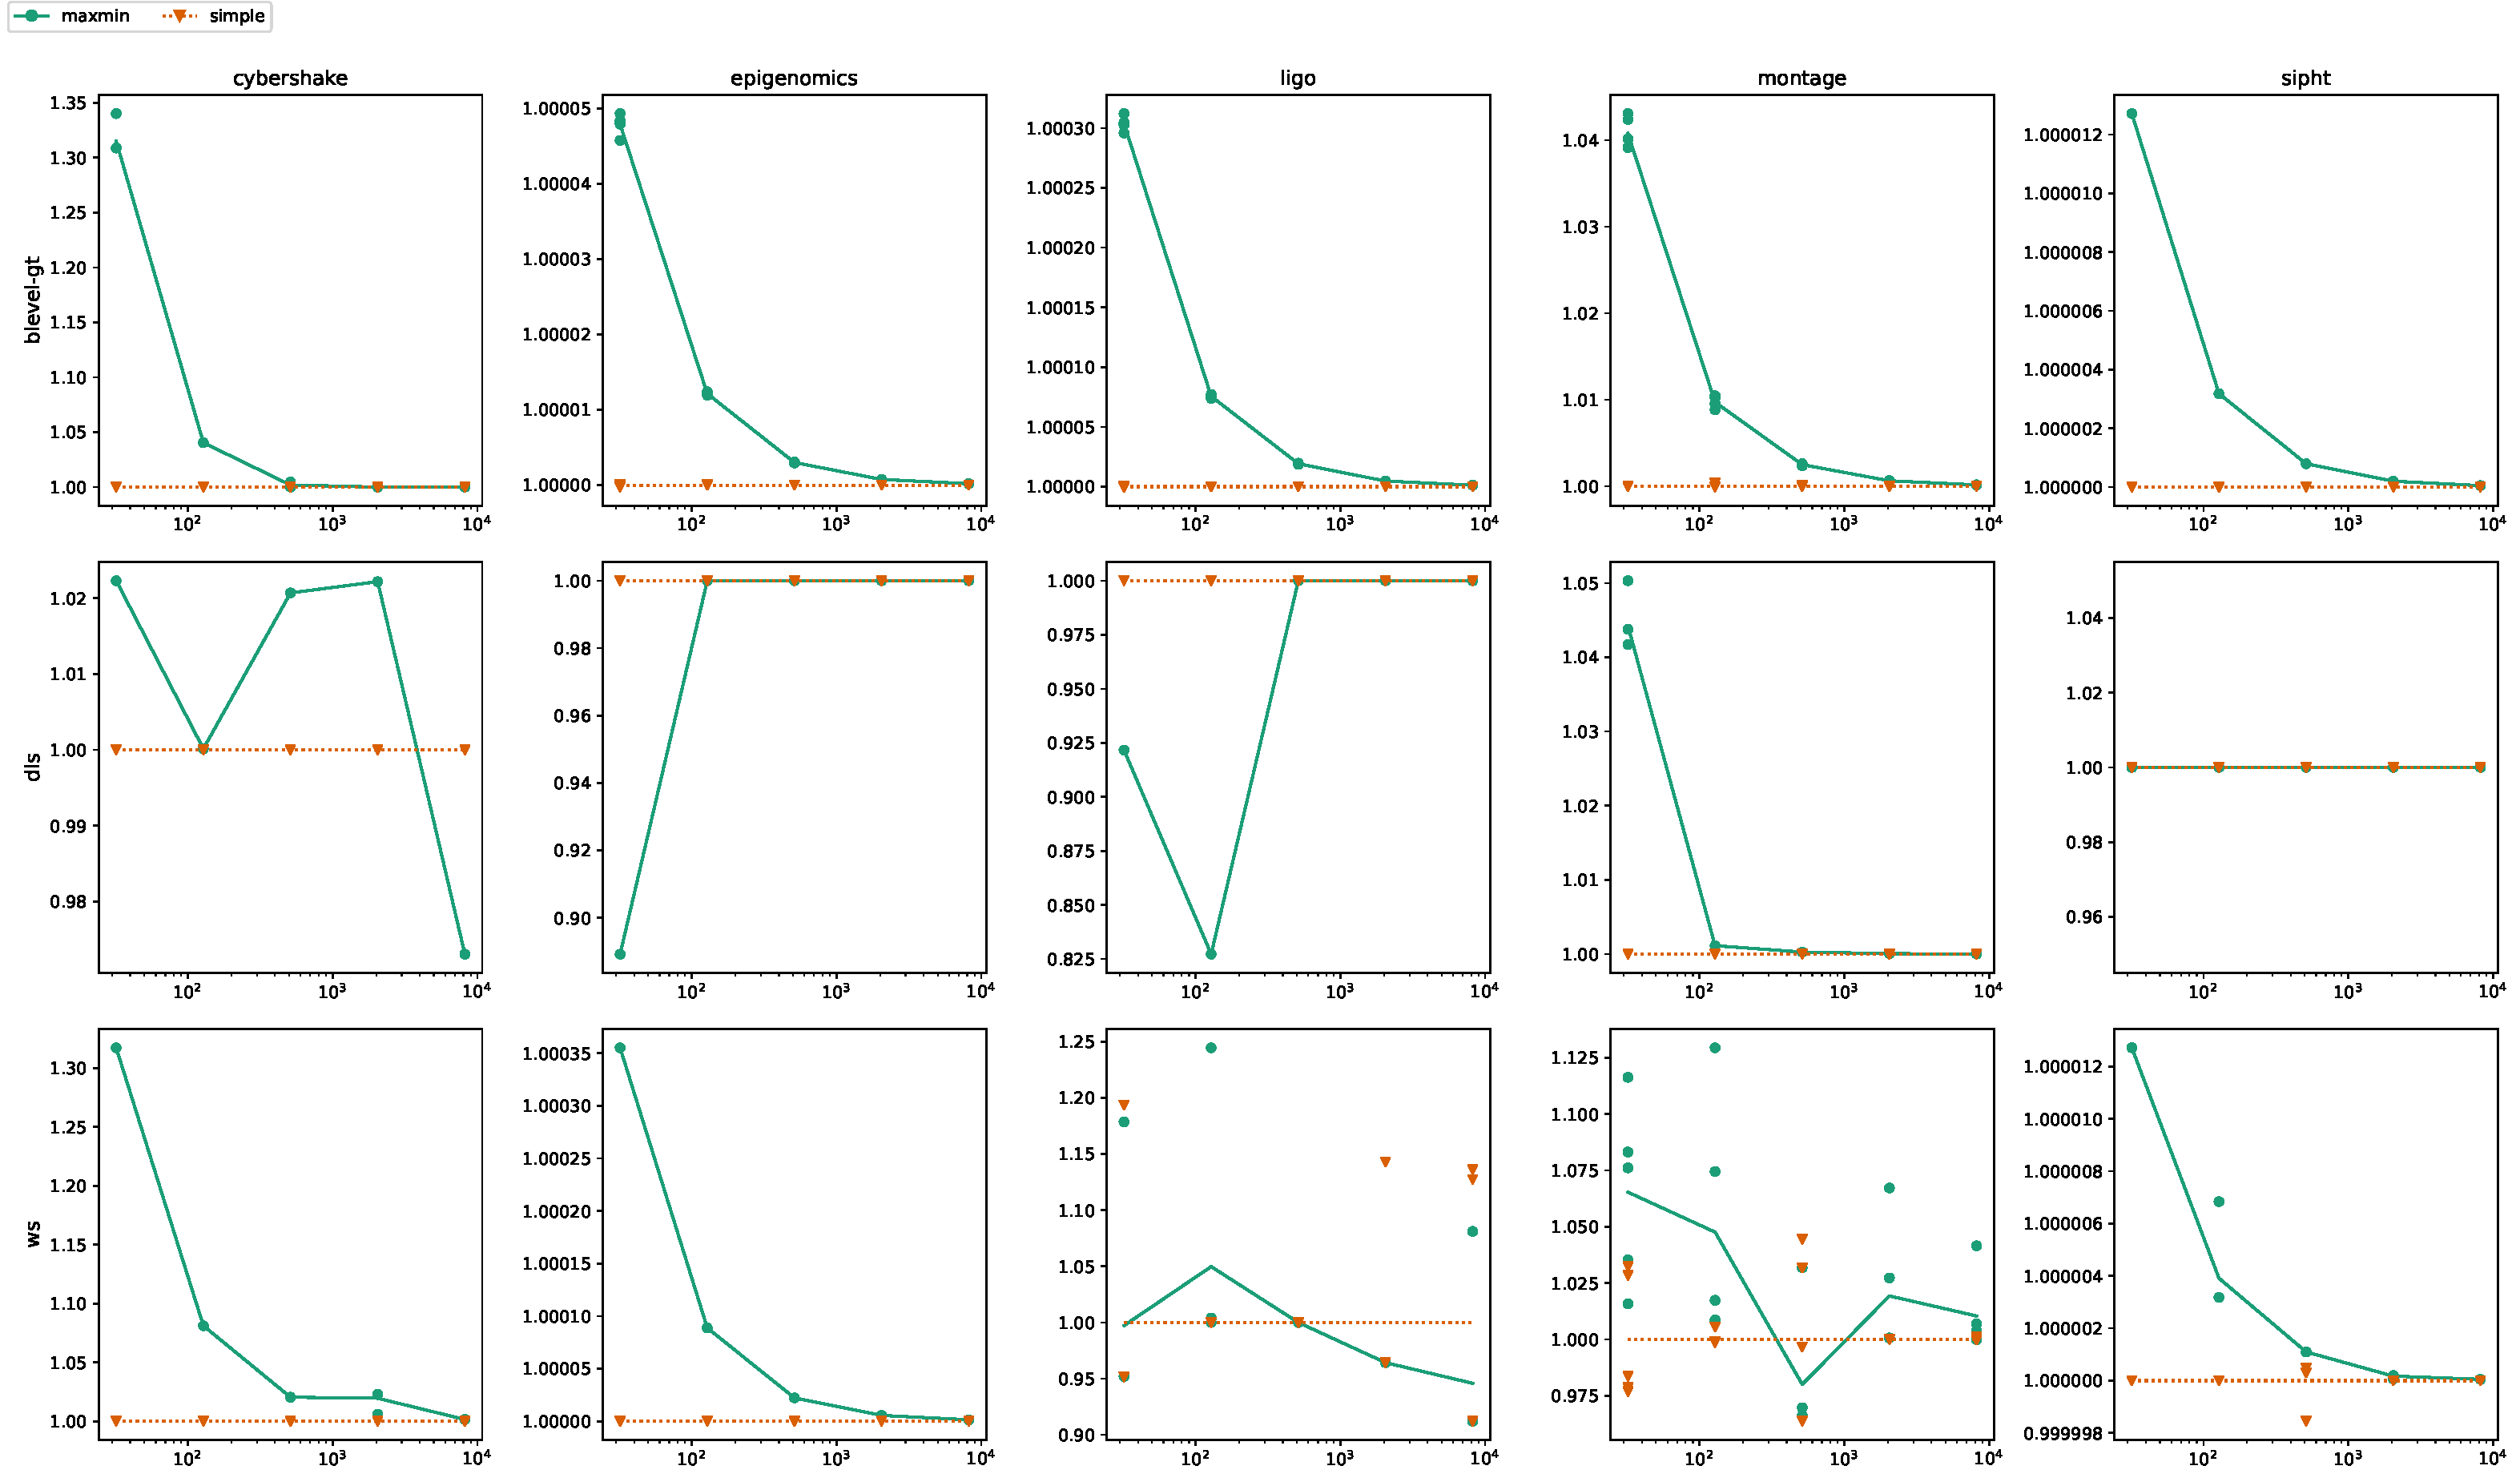
\includegraphics[width=\textwidth]{imgs/estee/charts/pegasus-32x4-netmodel-score}
%	\\ {\small horizontal axis: bandwidth [MiB/s]; vertical axis: execution makespan normalized
%	to average of the \emph{simple} model; row: scheduler, cluster
%	$32x4$} \caption{Comparison of \emph{maxmin} and \emph{simple} network models
%	(\emph{pegasus} dataset)} \label{fig:estee-chart-pegasus-netmodel}
%\end{figure}

\Autoref{fig:estee-chart-irw-netmodel} demonstrates how the used network model affects simulated task
graph makespans for a selected set of task graphs and schedulers, using task graphs from the
\emph{irw} dataset on the $32x4$ cluster with 32 workers. The Y axis
is normalized with respect to the average makespan of simulations performed with the
\emph{simple} network model.

It is clear that especially for slower network bandwidths, the naive \emph{simple} model
often underestimates the resulting makespan. This is caused by the fact that it does not take
network contention into account at all, which causes the overall network transfer duration
estimation to be overly optimistic. As network bandwidth goes up, the difference is reduced, since
there is less overall contention and the transfers are faster in general.

The makespans of simulations with these two network models are sometimes up to an order of
magnitude apart. This is quite significant, because the difference between the performance of
schedulers (with a fixed network model) is otherwise usually within a factor of two, which was
demonstrated both in~\cite{wang2018list} and by results of our other experiments. The gap
between the two network models depends heavily on the used task graph.
 %the difference was much smaller, as can be seen in~\Autoref{fig:estee-chart-pegasus-netmodel}.%For task graphs from the Pegasus dataset,

\subsubsection*{\acrlong{msd}}

\begin{figure}
	\centering
	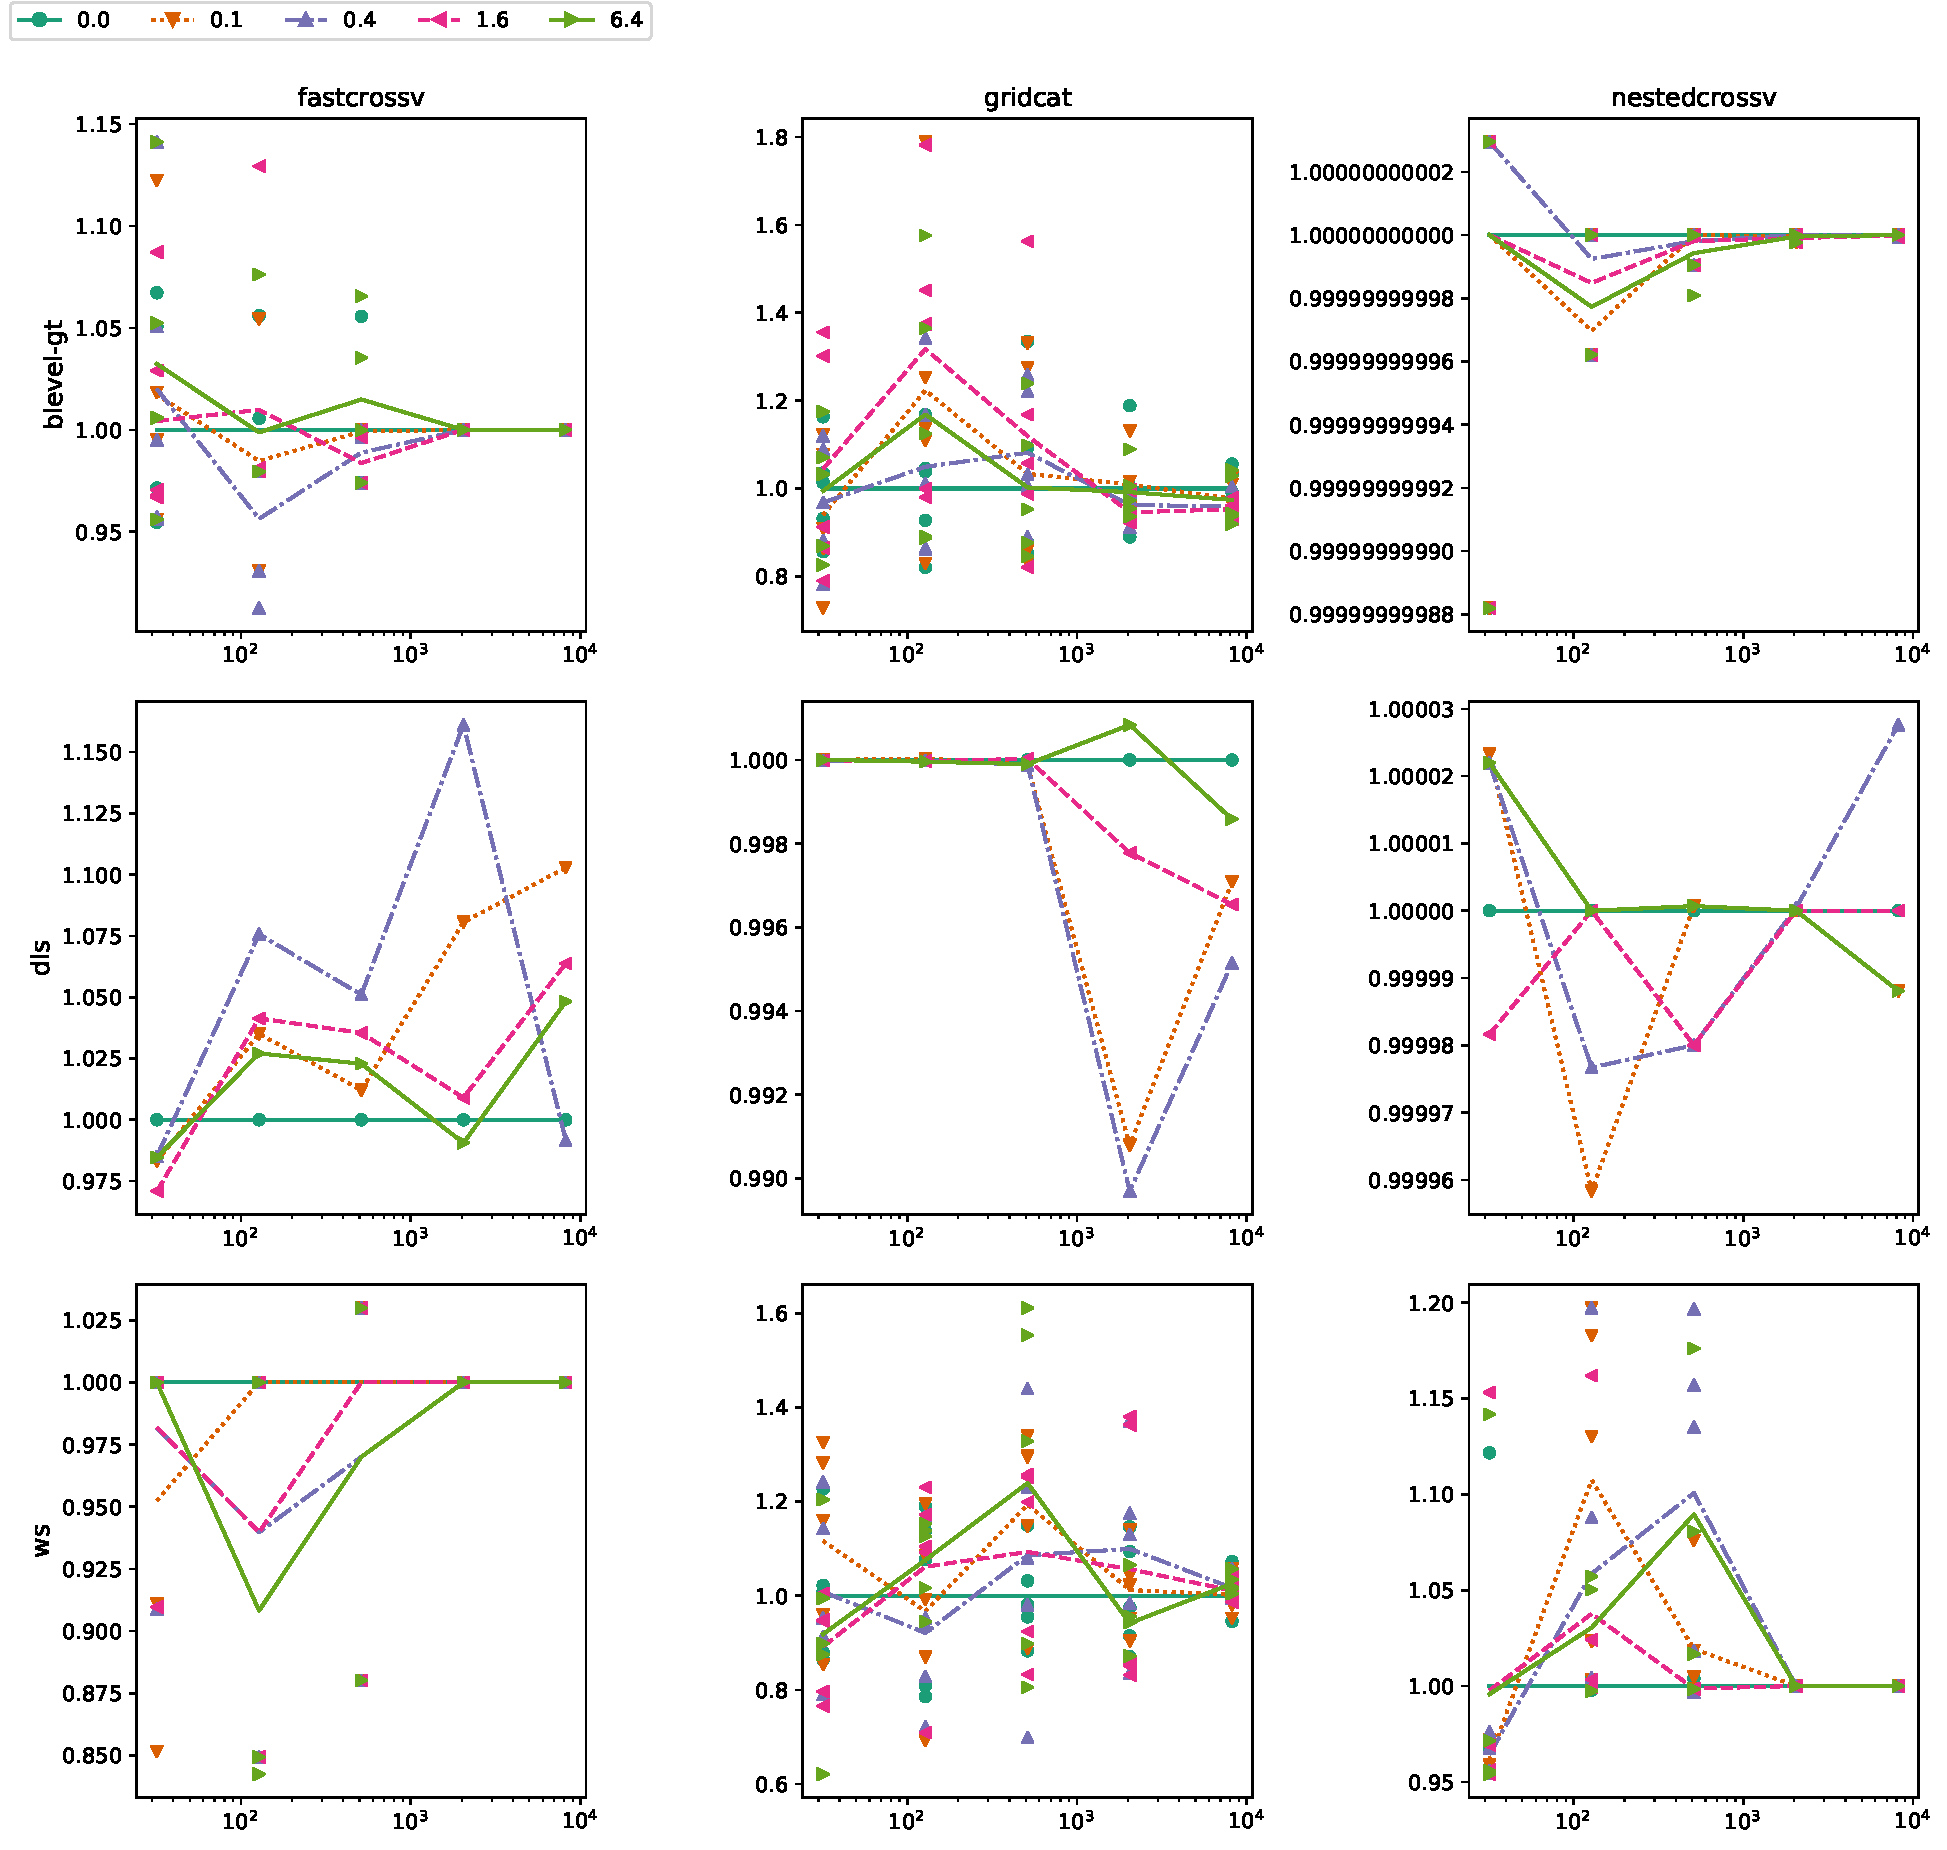
\includegraphics[width=0.8\textwidth]{imgs/estee/charts/irw-32x4-schedtime-score}\\
	{\small horizontal axis: bandwidth [MiB/s]; vertical axis: makespan normalized to
	$\gls{msd}=0$}
	\caption{Comparison of \acrshort{msd}; cluster 32x4}
	\label{fig:estee-chart-irw-msd}
\end{figure}

In~\Autoref{fig:estee-chart-irw-msd}, we can observe the effect of \gls{msd} on graphs from the
\emph{irw} dataset, with the $32x4$ cluster configuration. The Y axis
is normalized with respect to the configuration where \gls{msd} is zero. The results
show that the effect of \gls{msd} is relatively limited. There does not seem to be
any clear correlation or pattern that would suggest that a smaller \gls{msd}
consistently improves performance of a scheduler. Although interestingly, a higher
\gls{msd} value caused several makespan improvements, especially on the
\emph{gridcat} task graph.

This is another example of the non-trivial effect of scheduler heuristics. Increasing the
\gls{msd} leads to a batching effect, where the scheduler is allowed to make
decisions less often, but it has knowledge of more task events (that have arrived during the delay)
during each decision. Whether this helps its performance, or hurts it, depends on the specific
scheduler implementation and the task graph that it executes.

\subsubsection*{Information modes}

\begin{figure}
	\centering
	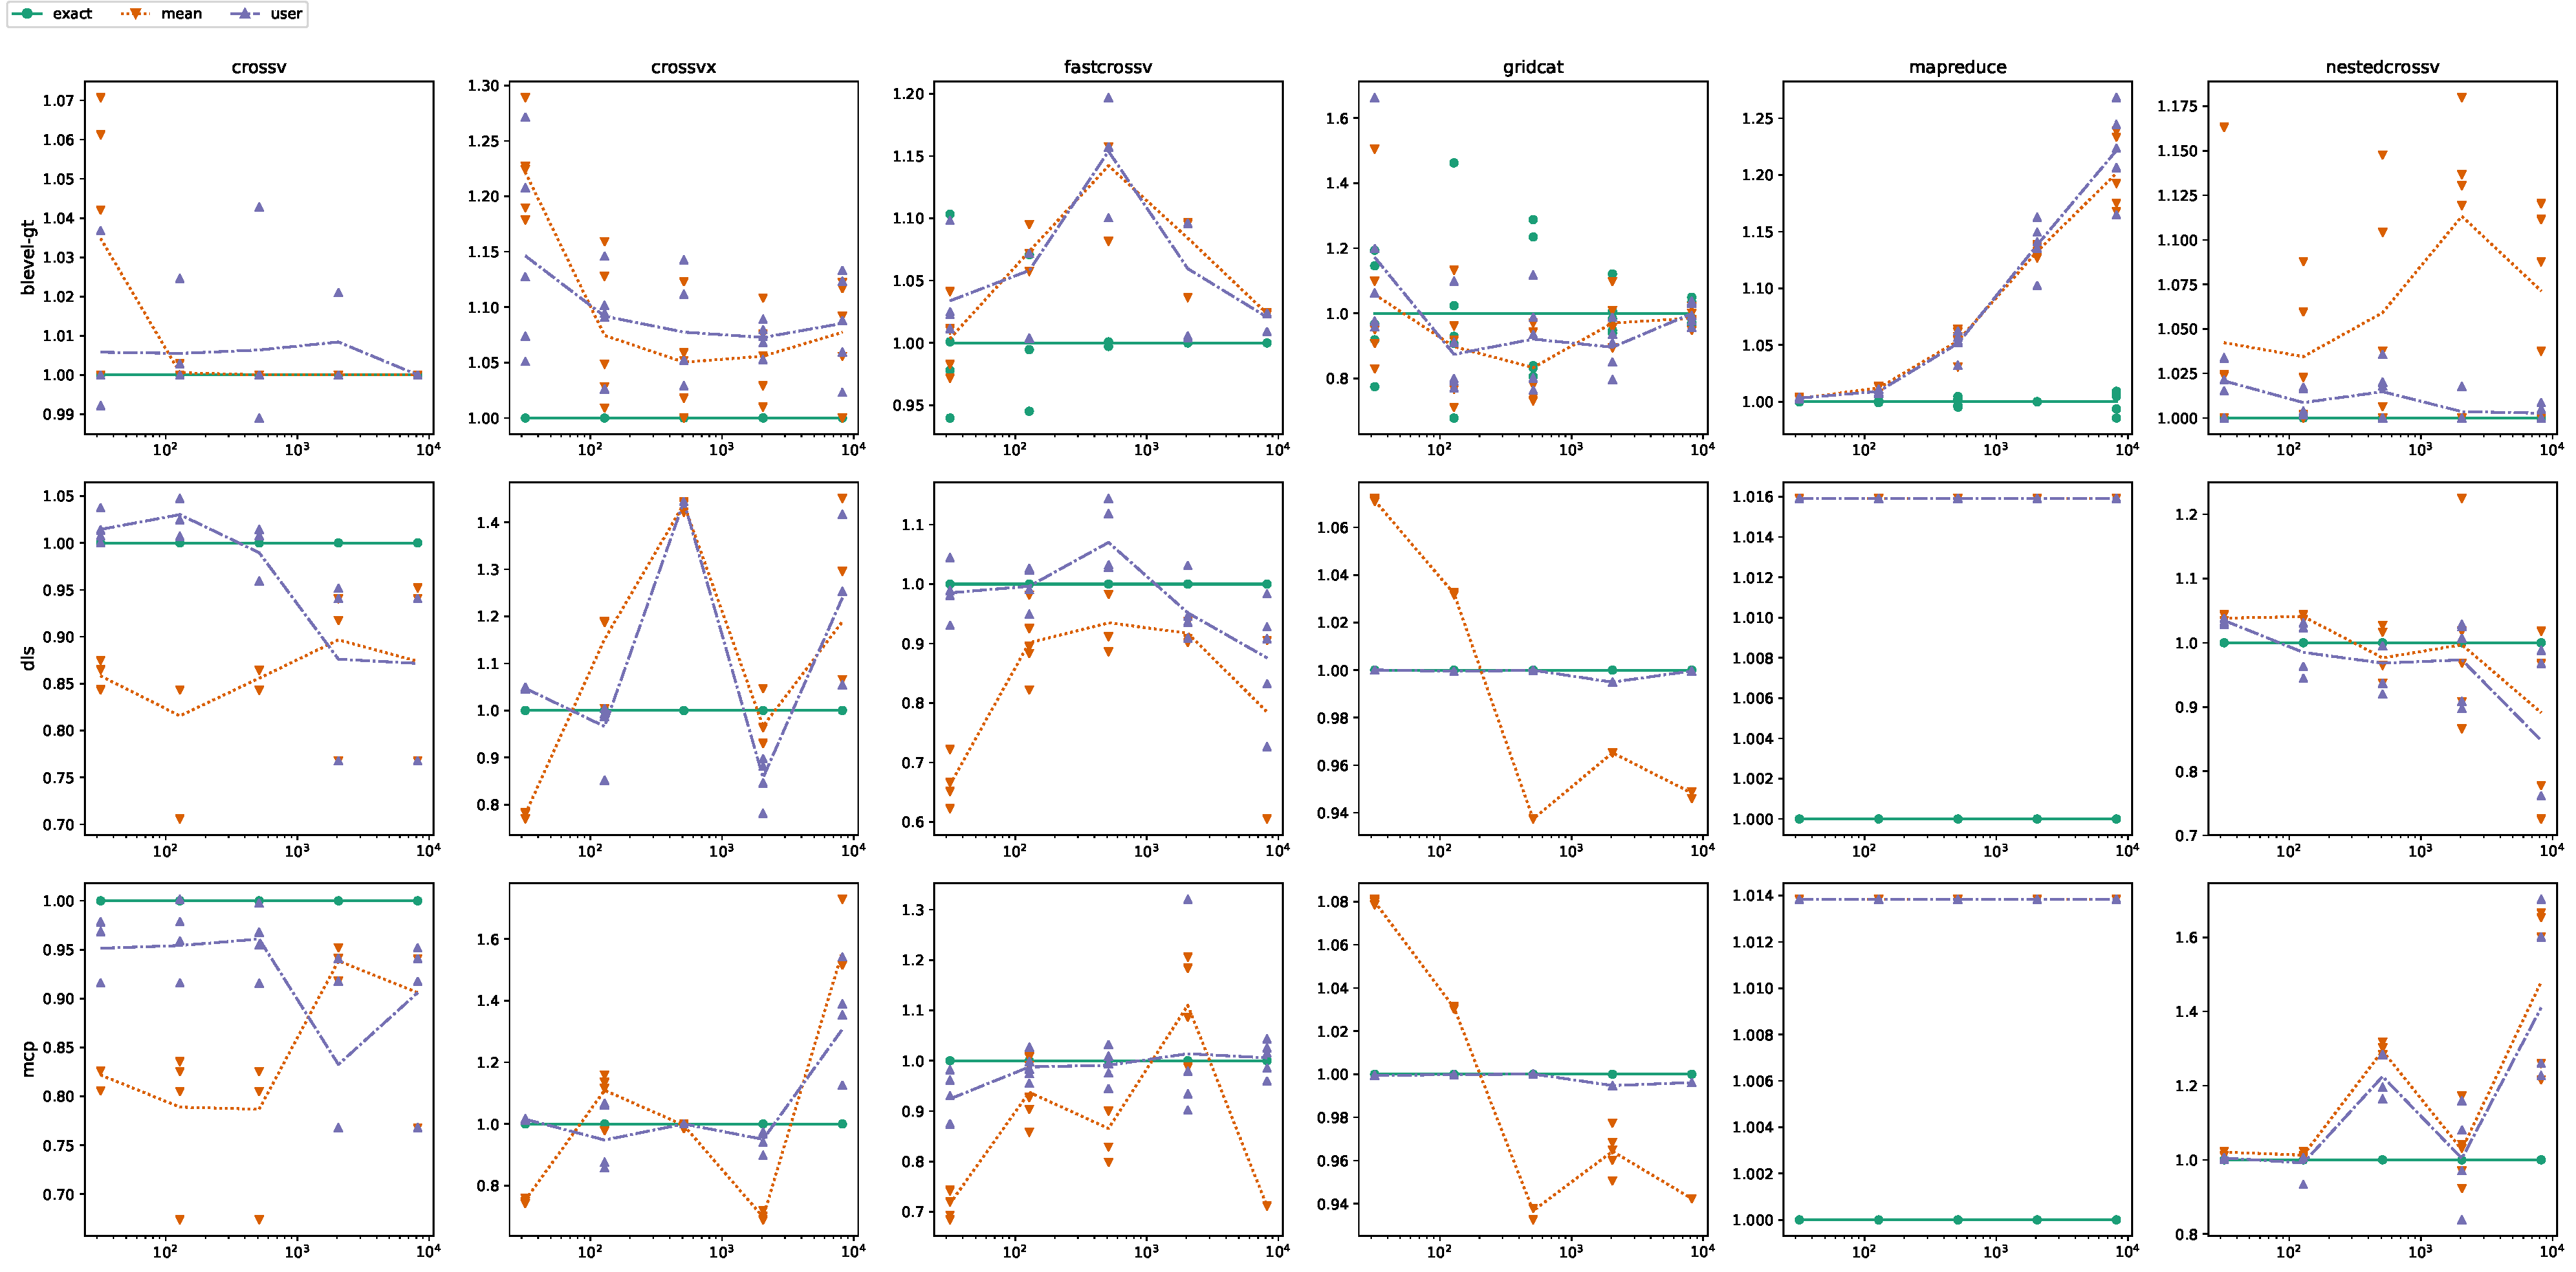
\includegraphics[width=\textwidth]{imgs/estee/charts/irw-32x4-imode-score}\\
	{\small horizontal axis: bandwidth [MiB/s]; vertical axis: makespan normalized to
	\emph{exact}
	imode; row: scheduler; cluster $32x4$} \caption{Comparison of information modes (\emph{irw} dataset)}
	\label{fig:estee-chart-irw-imode}
\end{figure}

%\begin{figure}
%	\centering
%	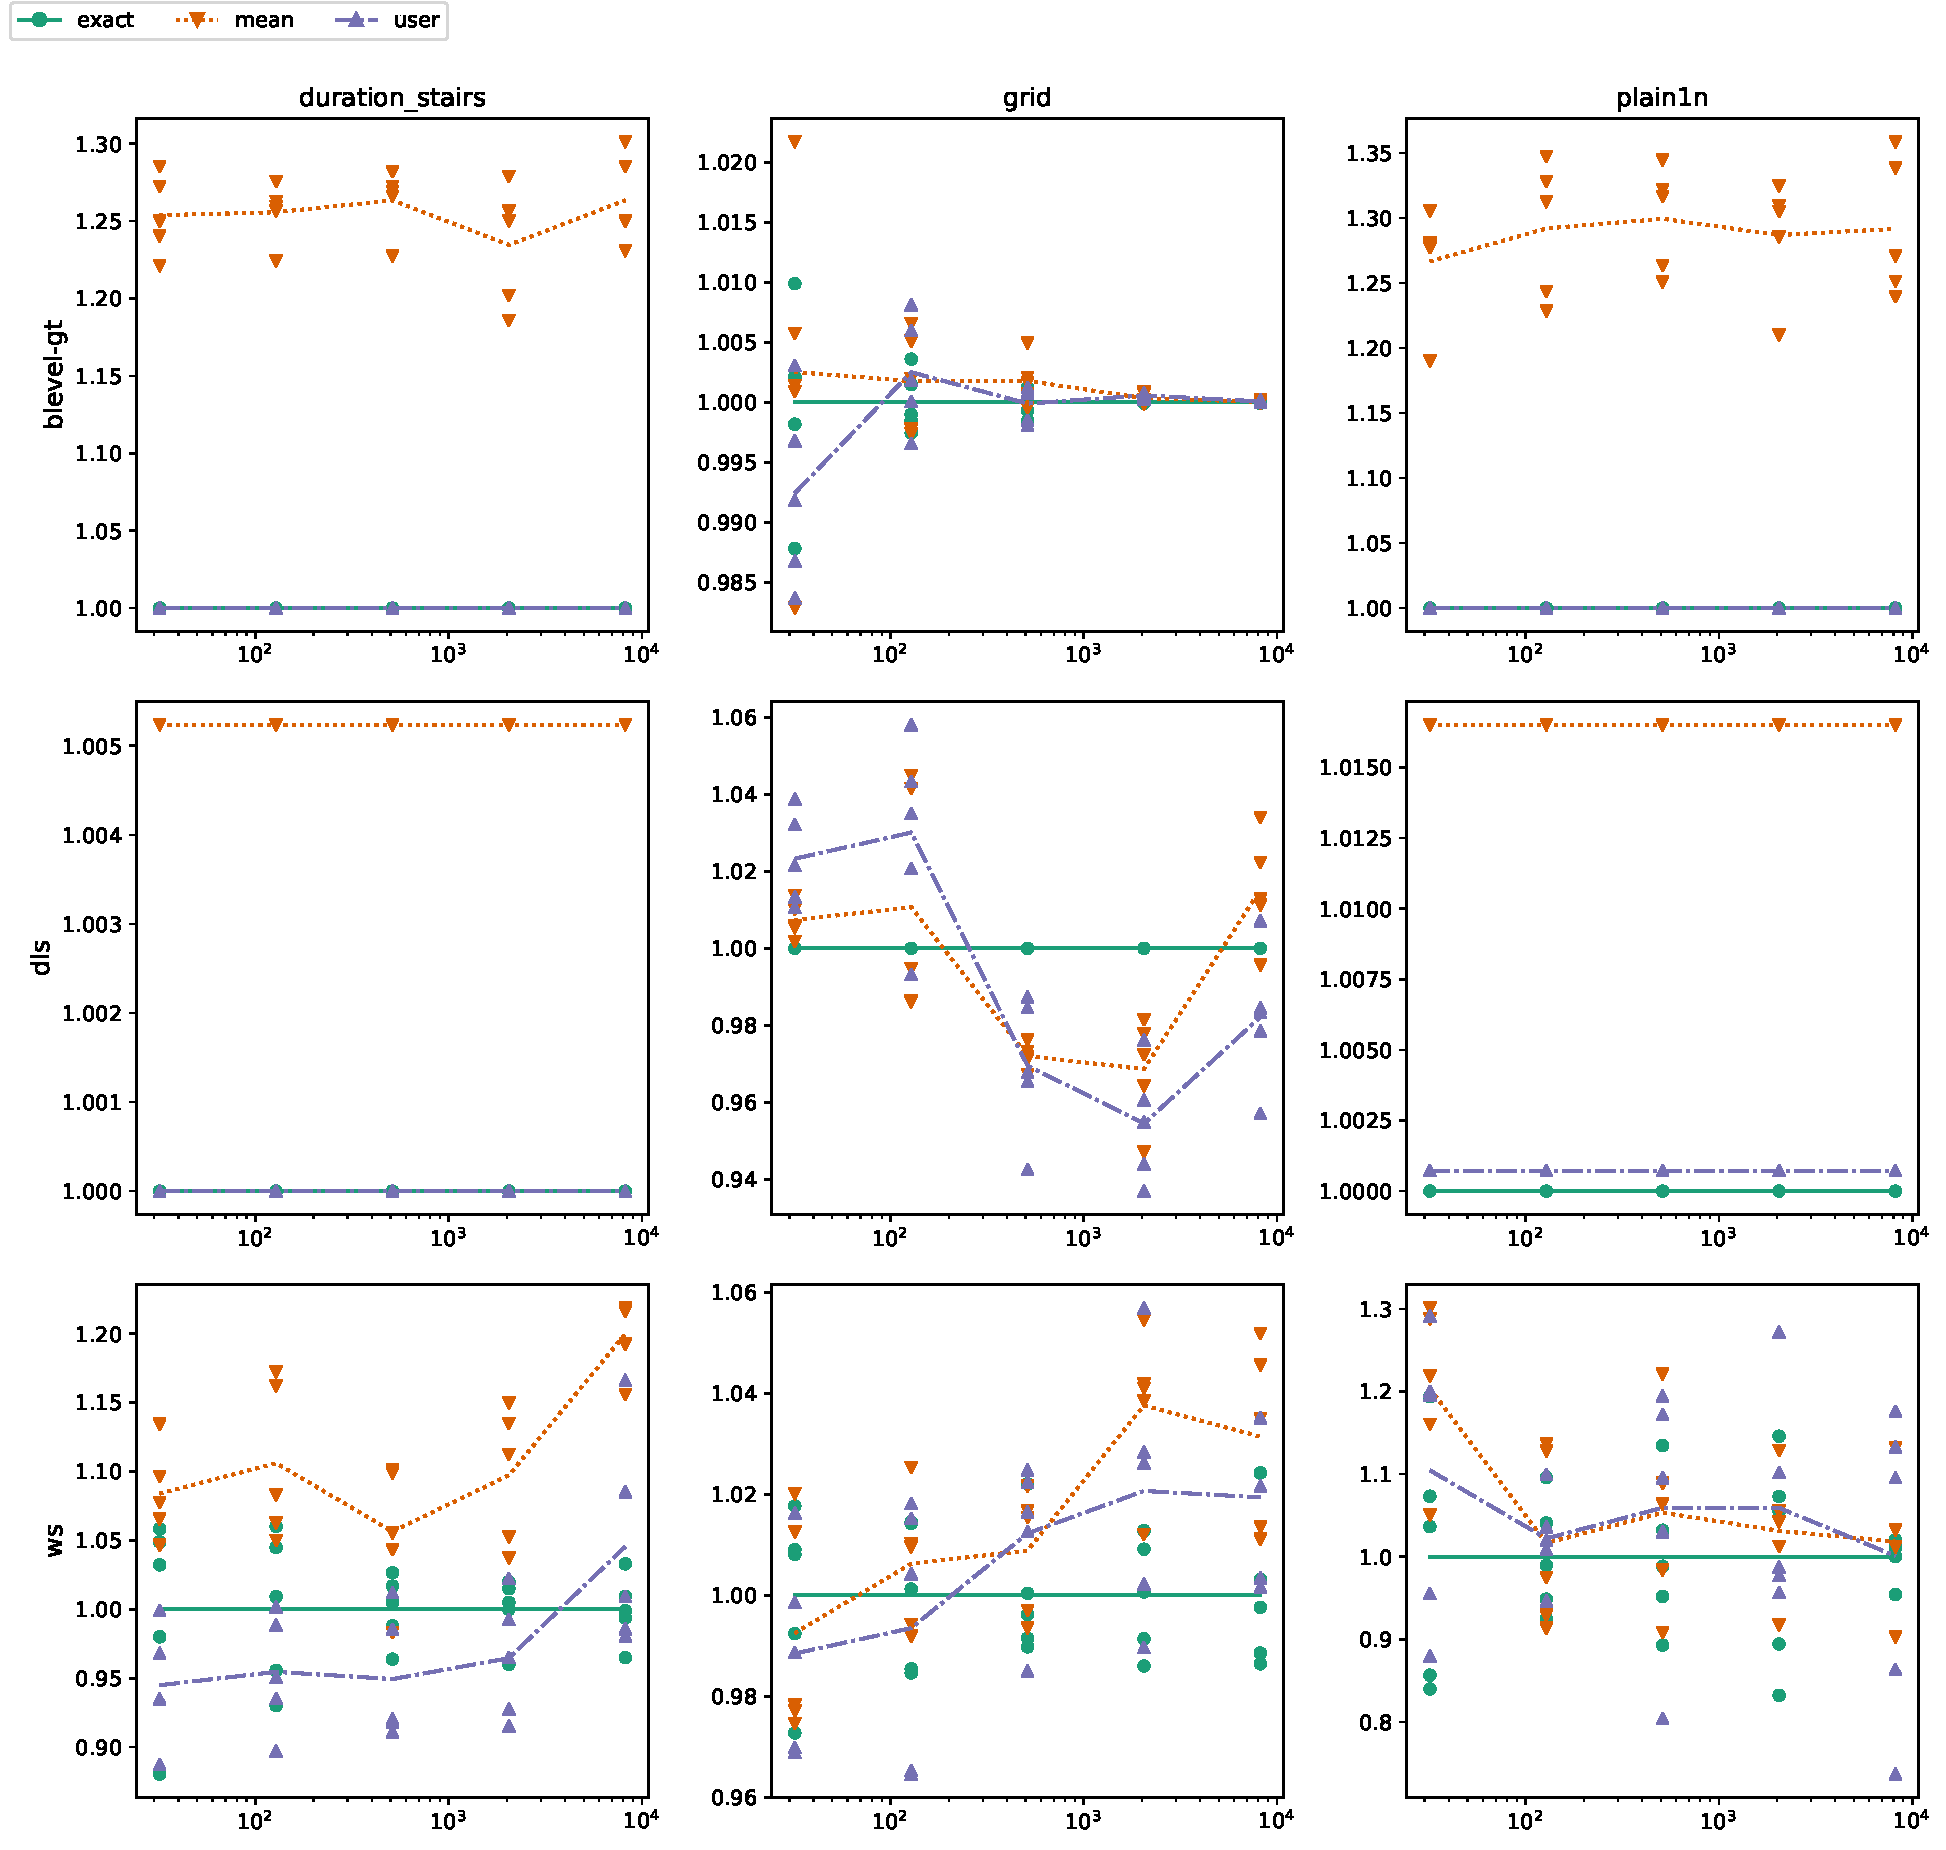
\includegraphics[width=0.8\textwidth]{imgs/estee/charts/elementary-32x4-imode-score}\\
%	{\small horizontal axis: bandwidth [MiB/s]; vertical axis: makespan normalized to
%	\emph{exact} average; row: scheduler; cluster $32x4$}
%   \caption{Comparison of information modes (\emph{elementary} dataset)}
%   \label{fig:estee-chart-elementary-imode}
%\end{figure}

\Autoref{fig:estee-chart-irw-imode} compares makespans of several scheduler and task graph combinations
from the \emph{irw} dataset on a $32x4$ cluster, with different
information modes being used. The results are normalized to the mean makespan of the default
\emph{exact} information mode. In general, the effect of information modes is more
significant than the effect of the \acrlong{msd}.

An intuitive expectation would be that with more precise task duration information, the scheduler
will be able to produce a shorter makespan, and this is indeed what happens in several cases, e.g.\
on the \emph{mapreduce} and \emph{nestedcrossv} task graphs with the
\emph{blevel-gt} scheduler, where the makespan is up to 25\% longer when task durations are
not exactly known.

However, there are also opposite cases, for example the \emph{dls} and
\emph{mcp} schedulers produce better results on several task graphs when they take
only the \emph{mean} task duration into account. This further shows the effect of
scheduler heuristics, which can produce worse results even when presented with more accurate data
input (and vice versa).

One factor that makes it more difficult for the scheduler to accurately estimate the network
transfer durations and thus make optimal use of the knowledge of task durations is that with the
max-min network model, the scheduler knows only a lower bound on the communication costs, even if
it knows the exact data size in advance. While it has access to the maximum bandwidth of the
network, it does not know the current (and most importantly, future) network utilization; thus it
has only a crude estimation of the real transfer duration.

\subsection{Validation}
It is challenging to validate the performance of different task schedulers in actual
(non-simulated) task runtimes. Schedulers tend to be deeply integrated into their task runtime in
order to be as performant as possible. That makes it difficult, or even infeasible, to replace the
scheduling algorithm without also modifying large parts of the task runtime. Furthermore, some
scheduling approaches might not even be compatible with the architecture of the runtime as a whole.
For example, work-stealing schedulers perform a lot of communication between the server and the
workers (potentially even between the workers themselves), and if the runtime does not implement
the necessary infrastructure for facilitating these communication patterns, then implementing a
work-stealing scheduler into such a runtime might amount to rewriting it from scratch.

In order to at least partially validate our simulation results, we have decided to use a modified
version of the \dask{}~\cite{dask} task runtime as a validation
framework. Apart from validating results from the \estee{} simulations, we have also
used this modified version of \dask{} to perform other experiments and benchmarks
that are described in~\Autoref{ch:rsds}, which also depicts the architecture of
\dask{} and our performed modifications in detail.

\dask{} is written in Python, which makes it relatively easy to modify and patch.
It uses a work-stealing scheduler by default, and even though it is relatively deeply integrated
within the \dask{} runtime, we were able to implement three simple alternative
scheduling algorithms into it\footnote{The modified version of \dask{} with these implemented schedulers can be found at
\url{https://github.com/Kobzol/distributed/tree/simple-frame-sched}.}, which correspond as closely as possible to
the \emph{random}, \emph{blevel} and \emph{tlevel} schedulers from
\estee{}. The default work-stealing scheduler was compared with our work-stealing
implementation of the \emph{ws} scheduler.

Apart from implementing new schedulers into \dask{}, there were several issues that
we had to solve to make sure that the comparison between the simulated and the real environment is
as fair and accurate as possible.

The absolute makespans of task graphs simulated by \estee{} and task graphs executed
by \dask{} cannot be compared directly, because there are many aspects of the
operating system, network, implementation of \dask{} itself and system noise that
\estee{} can not fully simulate. Therefore, since the primary goal of our task
scheduler experiments was to compare the relative performance of individual schedulers, we have
decided to compare the relative makespans normalized to a reference scheduler
(\emph{blevel}), to test if the makespan ratios between the schedulers is similar in
simulation and in real execution.

In the scheduler benchmarks, we have used many task graphs generated by the \estee{}
task graph generator. However, it would not be possible to perfectly replicate task durations of
these generated graphs in \dask{}. Therefore, we have approached this problem from
the other direction. We have executed several task graphs in \dask{}, and recorded
their execution traces, so that we would have a completely accurate representation of all the
executed task durations and data object sizes, which we could then accurately replicate in the
simulated \estee{} environment. The recorded task graphs will be described
in~\Autoref{sec:rsds-dask-overhead-analysis} and they can also be found in~\cite{rsds}. We have
executed these workflows with a $24x2$ cluster ($24$ cores on two nodes), which corresponds
to two nodes of the Salomon~\cite{salomon} cluster, on which were the \dask{} workflows executed.
Each actual execution and simulation was performed three times.

\begin{figure}
	\centering
	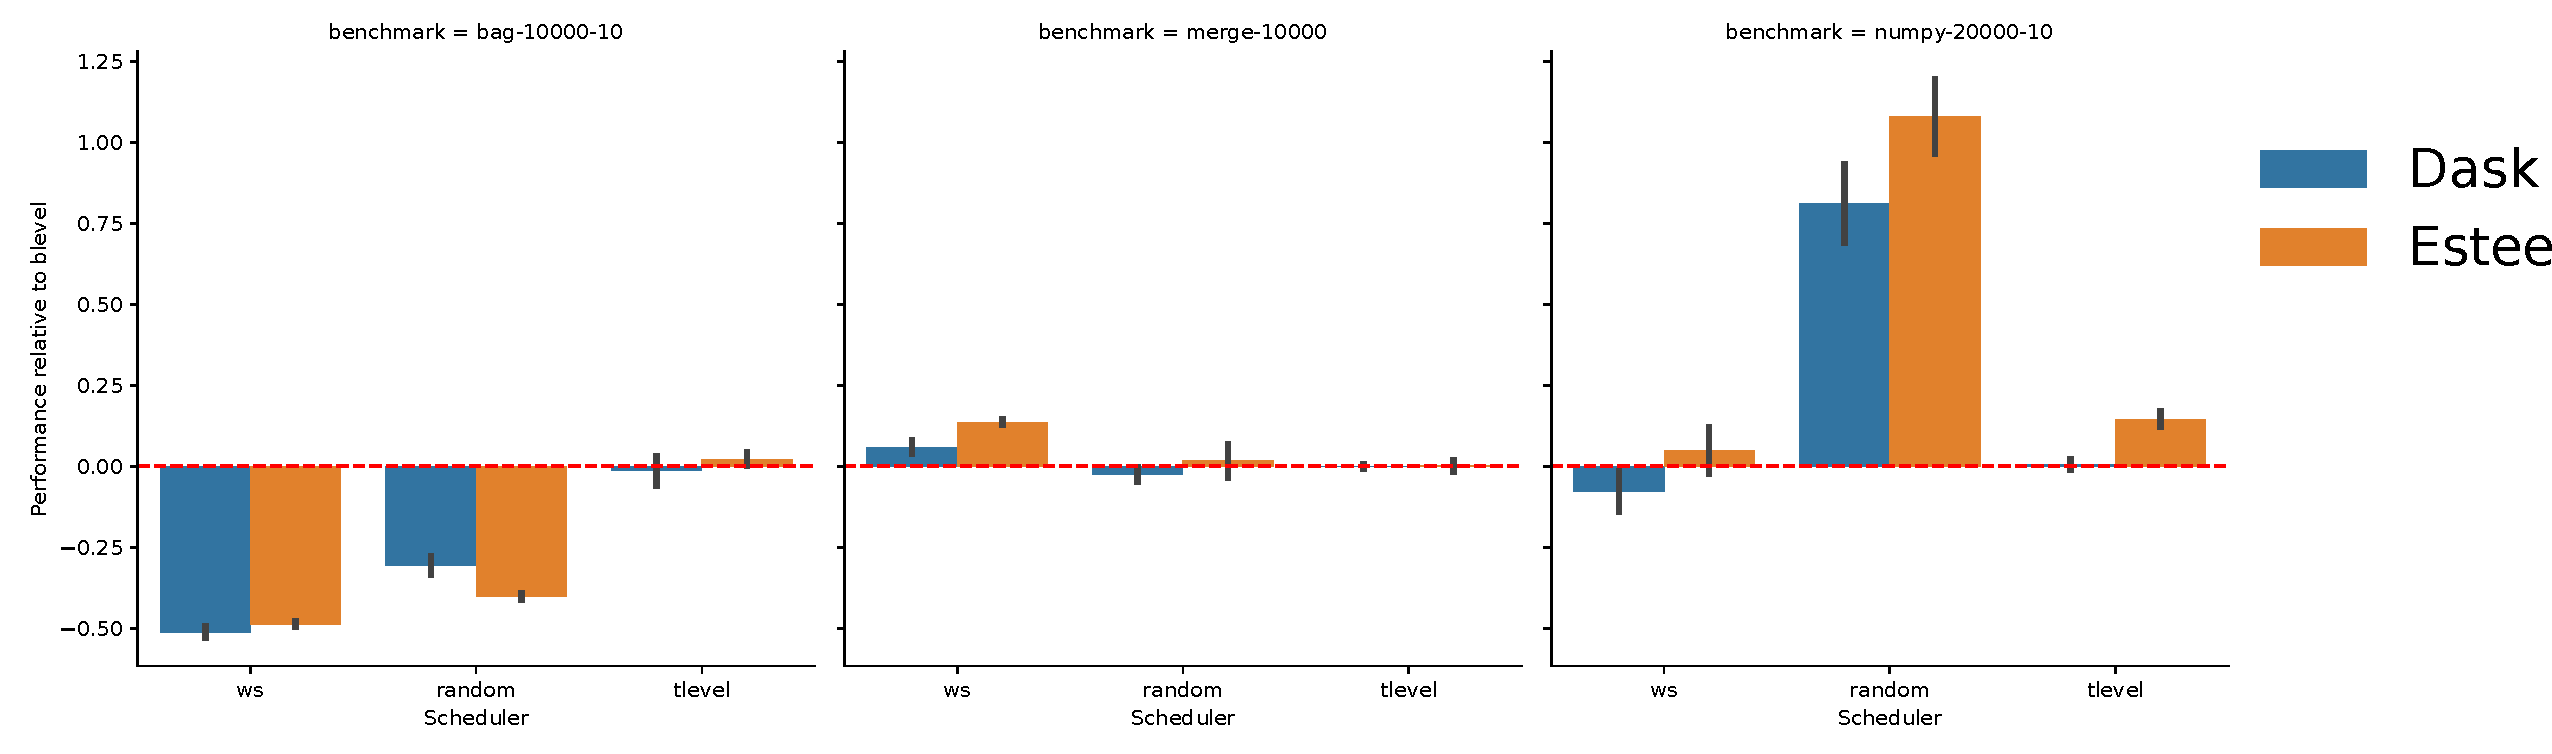
\includegraphics[width=\textwidth]{imgs/estee/charts/estee-validation}\\
	\caption{Scheduler performance relative to \emph{blevel} in \dask{} and \estee}
	\label{fig:estee-validation}
\end{figure}

\Autoref{fig:estee-validation} shows the results of the validation comparison for three selected
task graphs\footnote{Extended validation results can be found in~\cite{estee}.}. The performance of each scheduler was normalized to the
makespan of the \emph{blevel} scheduler within the same environment (either
\estee{} or \dask{}). Note that the relative ratios were centered
around zero by subtracting $1$ from them, to focus on the relative differences.
For example, if a task graph execution had a makespan of \SI{100}{\second} with the \emph{blevel} scheduler, but \SI{110}{\second} with the \emph{ws} scheduler, the ratio of the \emph{ws} scheduler would be
$0.1$. If the simulation was perfect, the two columns for each scheduler would
have the same height.

The first chart shows a situation where changing the scheduler resulted in large changes in
makespans, and \estee{} was able to simulate these changes relatively accurately, and reflect
the results measured in \dask{}. The second chart demonstrates a situation where
all schedulers produce similar makespans; therefore, in this case the scheduling algorithm does not
seem to be that important. \estee{} was again able to estimate that the differences
between schedulers will be small. In the third chart, we see that \estee{} was
systematically overestimating the makespans of all three schedulers (with respect to the reference
scheduler). The most important difference was in the \emph{ws} scheduler, where the
simulated result claims that it is slower than \emph{blevel}, while in reality it was
slightly faster. The work-stealing implementation in \dask{} is complex, and in
this case it was able to outperform \emph{blevel} in a way that \estee{}
was not able to simulate.

To summarize the average error of the simulated results, we took the relative makespans of the
individual schedulers w.r.t.\ the reference \emph{bevel} scheduler, and calculated the
difference between the executed and simulated relative makespan. The geometric mean of these
differences across all measured benchmarks was $0.0347$, which suggests that the
differences between the execution and simulation were relatively small; the simulated makespans
were usually within just a few percent off the actual makespan duration.

\section*{Summary}
We have implemented a set of well known scheduling heuristics, prepared a benchmark dataset
containing task graphs of different types and scales and designed a simulation environment for task
scheduler experimentation. We have conducted a series of reproducible benchmarks using that
environment, in which we have analyzed the effect of network models, minimal scheduling delays,
information modes and worker selection strategy on the behavior of the implemented schedulers, and
also compared their relative performance.

Our attempts to implement existing scheduling algorithms in \estee{} and reproduce
the results of previous scheduler benchmarks have shown that various implementation details which
are often missing from the algorithm's description (like the precise worker selection strategy) can
have a large effect on the final performance of the scheduler. Furthermore, we have been able to
confirm our hypothesis that the naive network model used in several existing works can result in
very inaccurate simulation results.

Combined with the fact that the source code of many published scheduling algorithms or surveys is
not open-source, it is difficult (even nigh impossible) to accurately reproduce their performance
results. We have tried our best to make all available source-code, benchmark datasets and the
results of our experiments public, to make them easy to reproduce and thus avoid this issue.

%Our analysis has shown that despite its simplicity, the foundational \gls{hlfet}
%algorithm~\cite{hlfet1974} (\emph{b-level}) produces high quality schedules in various scenarios and should
%thus serve as a good baseline scheduler for task runtimes. It can be complemented with
%work-stealing, which is able to dynamically react to load imbalances of individual workers.

We have demonstrated that even a completely random scheduler can be competitive with other
scheduling approaches for certain task graphs and cluster configurations.
This supports the conclusion made in~\cite{wang2018list}, where the authors have also observed
that relatively simple scheduling algorithms can be competitive, and more complex algorithms are
useful mostly for special situations and edge cases, where the simple heuristics might fail to
produce reasonable results.

The \acrlong{msd} had a smaller effect in our simulations than we have expected. This
hints that it might be possible to reduce the scheduling overhead (by invoking the scheduler less
often) without sacrificing schedule quality, but this will be highly dependent on the specific task
runtime implementation.

The effect of different information modes turned out to be significant, although it is unclear
whether schedulers can leverage the additional information about exact task durations when facing
unpredictable network conditions.

The implemented \estee{} simulator enables simple prototyping of task schedulers and
also allows simulating execution of various task graphs. We hope that it could have further
potential to simplify the development and evaluation of novel task schedulers.

Through our experiments presented in this chapter, we have learned more about the effect
of scheduling algorithms on the performance of task graphs. We have identified a
performant baseline scheduling approach, work-stealing combined with the \emph{b-level} heuristic,
which we have further leveraged in work described in the following two chapters.

Although task scheduling is an important factor, it is not the only aspect that contributes to the
overall overhead and performance of task runtimes. The following chapter will examine
the runtime overhead and scalability of a state-of-the-art task runtime in more detail.
